\chapter{The noun phrase}
\label{sec:NP}

\section{Introduction}
\label{sec:NPIntro}




Noun phrases can be viewed in relation to their syntactic status within a clause as well as to their internal structure. The status of a noun phrase within a sentence relates to its function as an argument (or else, for example as an adjunct) in relation to a predicate. The internal structure relates to questions such as ``What elements do noun phrases contain?'' and ``What is the order of these elements in a noun phrase?''  

\subsection*{The noun phrase on the sentence level} This latter perspective is usually assumed when defining the term ``noun phrase''. A definition depends, at least to some extent, on the function that is attributed to the noun phrase. \citet[132]{andrews2007} points out that there are three ways to think of functions of the noun phrase, namely in terms of its pragmatic, semantic,  or grammatical functions.

Pragmatic functions relate to information structure and include core notions such as ``topic'' and ``focus''. Information structure will be discussed in \sectref{sec:IS} since, first, information structure has to be seen on a phrase or even discourse level. Second, focused or topicalized elements of a phrase exceed noun phrases; for instance, verbs can also be the topic or focus of a sentence.

Semantic roles are imposed on noun phrases by predicates that create a certain situation and imply certain ways in which noun phrases participate as actors in this situation. They are called ``arguments'' to the predicate. \citet[135]{andrews2007} gives the example of the verbal element {\itshape kill} that requires a participant that takes over the role of the {\itshape killer} and one that is the {\itshape killed}.  Traditionally, there are general classes of semantic roles such as {\itshape agent}, {\itshape patient}, {\itshape recipient}, {\itshape experiencer} and many more.\footnote{See \citet{jackendoff90}, \citet{andrews2007}, and \citet{levin2005} for further readings on semantic roles.} 


\hspace*{-2pt}In terms of their grammatical functions, \citet[151]{dryer2007} defines noun phrases as ``syntactic constituents which serve as arguments of verbs''. They express core grammatical relations such as ``subject'' and ``object''. Classes of semantic roles relate in a systematic way to grammatical roles. Thus, very often, agents are the subjects of a sentence while patients are found in the object position.

\hspace*{-.5pt}These different grammatical relations can be expressed in different ways across languages. \citet[141]{andrews2007} posits ``three basic techniques which languages use to code syntactic functions: order and arrangement, {\NP}-marking, and cross-referencing''.  These different coding strategies will be discussed in detail in \sectref{sec:SC}.

It is important to make the distinction between semantic and grammatical functions of noun phrases and be aware of their relation. In this grammatical description of Gyeli, I adopt, however, an approach that focuses on a grammatical rather than a semantic description.

\subsection*{The internal structure of noun phrases} Having introduced the main functions of noun phrases on a sentence level as discussed in the literature, I now turn to noun phrases' internal constituency. \citet[23]{rijkhoff2002} points out that noun phrases vary in terms of their constituency and complexity, both within and across languages.\footnote{He further states that spoken languages (such as Gyeli) seem to be grammatically less complex than written languages, a claim that does not hold for Gyeli, which seems to be just as complex as neighboring Bantu languages that are taught at school.} \citet[151]{dryer2007} distinguishes different  types of noun phrases for a typological discussion of noun phrases across languages, ranging from simple to more complex noun phrases: (i) simple noun phrases, which contain only pronouns or nouns plus simple modifiers such as articles, adjectives, demonstratives, or numerals, (ii) complex noun phrases, which contain more complex sorts of modifiers such as genitive or possessive modifiers and relative clauses, and (iii) various types of noun phrases which lack a head noun.




Noun phrases in Gyeli can be zero-expressed, which is possible for subject noun phrases (\sectref{sec:SBJ}), while the subject is cross-referenced through agreement on the \textsc{stamp} marker or copula in the predicate.

Simple noun phrases include pronouns (\sectref{sec:PRO}). Pronouns can occur bare in all types of noun phrases: subject, object, and oblique. Pronouns can combine with the contrastive suffix -{\itshape gà} (\sectref{sec:CONTRS}) and be followed by three modifiers, as shown in \REF{protemp1}.

\ea\label{protemp1}
\ea {\PRO} {\itshape mɛ́dɛ́} `self'
\ex {\PRO} -{\itshape ɔ́(nɛ́)gá} `other'
\ex {\PRO} -{\itshape ɛ́sɛ̀} `all'
\z
\z

Simple noun phrases also consist of bare nouns.\footnote{A detailed discussion of how referents of bare nouns in Gyeli are tracked is provided in \citeauthor{grimmforthb} (To appear).} Gyeli does not have articles and bare nouns can occur in subject, object, and oblique noun phrases. Bare nouns can combine in simple noun phrases with elements discussed in \sectref{sec:NAdjuncts}. Gyeli is a head-initial language and almost all modifiers, both agreeing and invariable, follow the noun. There are two exceptions, however: the negative polarity item {\itshape tɔ̀} `any'  (\sectref{sec:InvQUANT1} and {\itshape nyá} `big' always precede the noun. If a simple noun phrase includes more than one postnominal modifier, the order of the modifiers is freely variable,\footnote{It may be that a change in order results in a slightly different reading in terms of emphasis on one or the other modifier, but this was not clear from my data.} and there does not seem to be a particular modifier that is closer to the noun than others. The reason for this could be that multiple modifiers in simple noun phrases are highly dispreferred. Tests on modifier combinations in a simple noun phrase all stem from grammaticality judgment tests in elicitations. In natural texts, however, the only instance were two modifiers where combined in a noun phrase is given in \REF{protemp2}.

\ea\label{protemp2}
 \glll  bèsâ bíndɛ̀ byɛ́sɛ̀ \\
be-sâ bí-ndɛ̀ by-ɛ́sɛ̀ \\
be8-thing 8-{\ANA} 8-all \\
 \trans `all these things'
\z

Other simple noun phrases that include two modifiers (or elements that are treated like modifiers) are complex cardinal numerals which contain an underlying multiplication operation, as in \REF{NPNum}.

\ea\label{NPNum}
\ea \label{NPNum1}
  \gll     b-ùdì [mà-wúmɔ̀ má-báà] \\
                ba2-person {\db}ma6-ten 6-two \\
    \trans `twenty people'
\ex[*]{\label{NPNum2}
 \gll    [mà-wúmɔ̀ má-báà] b-ùdì \\
        {\db}ma6-ten 6-two ba2-person \\
    \trans `twenty people'}
\z
\z

\noindent The structure of \REF{NPNum1} is [N $[$N + Num$]$\textsubscript{MOD}]\textsubscript{NP}. While {\itshape mawúmɔ̀} `10s' is a noun itself, in this construction, the entire complex numeral behaves like one postnominal modifier, without agreeing with the head noun {\itshape bùdì} `people'.  It is not possible for the numeral {\NP} to precede the quantified head noun, as shown in \REF{NPNum2}. 


Complex noun phrases in Gyeli include distributive constructions and noun + noun attributive constructions. Also noun phrases including relative clauses fall in the category of complex noun phrases, according to \citet{dryer2007}. As they constitute a type of subordination, they are discussed in \sectref{sec:Relativeclauses}.   In the remainder of this chapter, I first outline the gender and agreement system of Gyeli. I then discuss complex noun phrases and conclude with a note on the semantic category of numerals. 









\section{The gender and agreement system}
\label{sec:Gender}

As a typical feature of a Bantu language, Gyeli has a relatively elaborate gender and agreement system. In the literature, this is often referred to as ``noun class'' or ``concord'' systems, depending on the authors' preferences and research tradition. Authors differ substantially in their definition of key notions such as ``noun class'' and ``gender''. Often, these terms are used interchangeably as in \citet[190]{heine82}:
\begin{quote}
A noun class or gender system is said to be present if the nouns of a given language are divided into classes by means of concordial agreement markers.
\end{quote}

\citet[19]{aikhenvald2003}, for instance, notices the widespread interchangeable use of ``noun class'' and ``gender'' and opts for adopting ``noun class'' as the generic term for both noun class and gender, while the term ``gender'' should be restricted to noun categorization systems that are sex-based, i.e.\ which make a distinction between grammatical {\itshape feminine} versus {\itshape masculine}. In that, she deviates from \citet{corbett91}, who uses the term ``gender'' for all agreement-based noun classification systems, both sex-based and non-sex-based systems alike.

Some authors, for instance \citet[85]{mve2011}, establish gender systems solely based on pairings of noun class prefixes rather than by agreement classes. This method artificially inflates the system since there are more pairings of noun class forms than agreement classes.
In light of such terminological confusion, I will first clarify the terminology I use before moving on to the description of the Gyeli system. I distinguish three terms:  ``agreement class'', ``gender'', and ``noun prefix class'', based on \citet{guldemann2019} in their straightforward approach to analyze noun categorization in a consistent way that facilitates cross-linguistic comparison.\footnote{\citet{guldemann2019} use the term ``nominal form class'' for the category that I call  ``noun prefix class''.} Prefixes that mark agreement are called ``agreement prefixes'', while prefixes that fall into the category of noun prefix classes are called ``noun prefixes''. 

\subsubsection*{Agreement class}  
According to \citet[13]{guldemann2000}, agreement class is defined by ``regular morphological processes on the parts of speech that are controlled by a particular noun in a given utterance". An agreement class thus consists of ``a set of noun forms that share an identical behavior across all agreement contexts of a given system'' \citep[98]{guldemann2019}. 
Following \citet{corbett91}, the parts of speech that agree with a noun are called ``agreement targets'', while the noun that controls agreement on depending parts of speech is called ``agreement trigger''. I label agreement classes in Gyeli by Arabic numbers, following the Bantuist tradition.

Agreement classes often conflate several grammatical features, such as gender and number. This is also true for Gyeli where the majority of nouns trigger one agreement pattern in the singular and a different pattern in the plural. There is also a transnumeral gender that lacks this singular/plural pairing and only has one agreement class. 

I take \posscitet[98]{guldemann2019} approach, in contrast to \citet{corbett91}, who point out that it is of ``no concern whether noun forms of one agreement class are of the same gender, number or any other feature''.  In Gyeli, for instance, most noun forms in agreement class 8 take a {\itshape be}- prefix and encode plurality, serving as the counterpart to the singular agreement class 7. There are, however, some exceptions where the noun form does not take the {\itshape be}- prefix, does not encode plural, but singular, and does not pair with agreement class 7, but agreement class 6. Nevertheless, because the agreement pattern is the same on all targets, this noun form still belongs to agreement class 8. 



\subsubsection*{Gender} Gender cannot be established by solely investigating the noun itself and potentially its changing affixes in the singular and the plural. Rather, the gender of a noun is exclusively established by agreement phenomena.
The term ``gender'' is widely discussed in the literature, especially by \citet[1]{corbett91}. He defines ``gender'' as ``classes of nouns reflected in the behavior of associated words'', citing \citet[231]{hockett58}. \citet[45]{corbett91} more specifically views ``gender'' as a ``set of nouns which take the same agreements (typically a singular-plural pair)''.  \citet[13]{guldemann2000} emphasizes that nouns are assigned to a nominal category ``according to some feature that is conceptually \textsc{inherent} to a  given noun'' and that ``noun gender refers to a more abstract item of the lexicon''.  As mentioned above, it is cross-linguistically frequent, especially in Bantu languages, that gender is conflated with number. \citet[98]{guldemann2019} point out that, analytically, gender classes ``are derived by abstracting from all other agreement features'', such as number. 
I label genders in Gyeli by their pairing of agreement classes, as discussed below. For instance, the noun -{\itshape ùdì} `person' inherently belongs to the class of nouns that triggers agreement class 1 in its singular form and agreement class 2 for the plural. It therefore belongs to gender 1/2.

The difference between agreement class and gender can be illustrated with an example from Gyeli.\footnote{The provided example is parallel to one that \citet[13]{guldemann2000} quotes from \citet[125]{nichols92} on Luganda.} A nominal root such as -{\itshape kɔ́ndyì} `hand' comes in two forms, namely as {\itshape le-kɔ́ndyì} in the singular and {\itshape ma-kɔ́ndyì} in the plural. The first triggers agreement of class 5, i.e.\ all dependent parts of speech will show the agreement pattern which belongs to this agreement class,  while the latter triggers class 6 agreement on all agreement targets. Thus, the nominal lexeme -{\itshape kɔ́ndyì} belongs to gender 5/6 which is a pairing of agreement classes 5 and 6. 



\subsubsection*{Noun prefix class} In many cases, the noun prefix reflects the agreement class that the noun triggers. For instance, the noun prefix {\itshape le}- in {\itshape le-kɔ́ndyì} `hand', is identical in form with most agreement targets such as subject marking, demonstratives, or the attributive marker (as shown in \tabref{Tab:AGRcl}). There are, however, also noun prefix classes which do not map onto their respective agreement classes. One example is the noun prefix class that is marked by a nasal N-. This noun prefix class is found both in agreement classes 1 and 3. At the same time, there are nouns of agreement classes 1, 3, 7, 8, and 9 that do not take any noun prefix at all. Unlike for genders and agreement classes, I refer to noun prefix classes not by numbering, but by the form of their prefix.
Since gender is determined only by agreement, noun prefix classes are not decisive in establishing gender or agreement classes. Noun prefix classes therefore relate to prefix marking on the noun but do not necessarily index agreement class affiliation.  

\subsection{Agreement targets of the noun}
\label{sec:AGRtargets}

Gyeli has a range of agreement targets, both within the noun phrase and noun phrase externally, as listed in \tabref{Tab:AGRtargetx}.  Each of the agreement targets is described in detail according to their part of speech in \chapref{sec:POS}, while agreement forms are listed in \tabref{Tab:AGRcl}.  


\begin{table}
\begin{tabularx}{\textwidth}{Xl}
 \lsptoprule
{Noun phrase internal} & Agreement taregts with agreement prefix \\
& ~~	Object pronouns \\
& ~~	Possessor pronouns \\
& ~~	Anaphoric markers \\
& ~~	-{\itshape vúdũ̂} `one' \\
& ~~	-{\itshape fúsì} `different' \\
& ~~	-{\itshape ɛ́sɛ̀} `all' \\
& ~~	-{\itshape ɔ́(nɛ́)gá} `other' \\
& ~~	Numerals `2' through `5' \\
& ~~	Genitive marker {\itshape ngá} \\
& ~~	{\itshape nyá} `big' \\
& Agreement targets with free agreement morpheme \\
& ~~	Subject pronouns \\
& ~~	Demonstratives \\
& ~~	Attributive markers \\  \midrule
{Noun phrase external} &   ~~	\textsc{stamp} marker \\
& ~~	Copula \\
 \lspbottomrule
\end{tabularx}
\caption{Agreement targets}
\label{Tab:AGRtargetx}
\end{table}




\subsection{Agreement classes}
\label{sec:AGR}

Gyeli has nine agreement classes that are reflected in the morphosyntactic behavior of their agreement targets. These agreement targets and their agreement patterns are listed in \tabref{Tab:AGRcl}.  Parts of speech that agree with a head noun in gender (and number) mark agreement either by free agreement morphemes or by agreement prefixes. Free agreement morphemes in Gyeli include the subject-tense-aspect-mood-polarity marker (\STAMP),\footnote{Subject marking is achieved by the subject-tense-aspect-mood-polarity (\textsc{stamp}) marker. Its forms are represented without tones because the surface tone depends on the tense-mood category (\sectref{sec:SCOP}) it encodes.} a copula, subject pronouns, demonstratives,\footnote{Demonstratives have two patterns with a distinction for proximal versus distal. In \tabref{Tab:AGRcl}, only the proximal demonstratives are shown as representatives of the whole paradigm.} and attributive markers (\sectref{sec:ATT}), which typically link two nouns in a possessive construction and also indicate an embedding relation between a relative clause and the modified noun phrase. 

Parts of speech that mark agreement through prefixes include object and possessor pronouns, anaphoric markers, nominal modifiers, the numerals `1' through `5', and the genitive marker, which only take agreement prefixes in plural agreement classes. 


\begin{table}
\begin{tabular}{l lllllllll}
 \lsptoprule
{\AGR} class   &  1 & 2 & 3 & 4 & 5 & 6 & 7 & 8 & 9 \\
\midrule
\multicolumn{10}{l}{Monomorphemic agreement words} \\
  {\STAMP} &  a/nyɛ/nu & ba & wu & mi & le & ma & yi & bi & nyi \\
  {\COP} &   àà/nùù & báà & wúù & míì & léè & máà & yíì & béè & nyíì \\
  {\SBJ} &   nyɛ̀ & bá & wú & mí & lí & má & yí & bé & nyì\\
  {\DEM} &   nû & bâ & wɔ̂ & mî & lê & mâ & yî & bî & nyî \\
 {\ATT} &  wà & bá & wá & mí & lé & má & yá & bí & nyá \\
\midrule
\multicolumn{10}{l}{Agreement prefixes} \\
 {\OBJ} &   nyɛ̂ & b-ɔ̂ & w-ɔ̂ & my-ɔ̂ & l-ɔ̂ & m-ɔ̂ & y-ɔ̂ & by-ɔ̂ & ny-ɔ̂ \\
 {\POSS} &   w- & b- & w- & mí- & l- & m- & y- & bí- & ny- \\
 {\ANA} &   nú- & bá- & wɔ́- & mí- & lé- & má- & yí- & bí- & nyí- \\
\textsc{mod}(-C) &   m- & bà- & m/$\emptyset$- & mì- & lè- & mà- & $\emptyset$- & bì- & m/$\emptyset$- \\   
 \textsc{mod}(-V) &  w/n- & b- & w- & my- & l- & m-  & y- & by- & ny- \\
 {\NUM}, {\GEN} &   - & bá- & - & mí- & - & má- & - & bí- & -\\
  \lspbottomrule
\end{tabular}
\caption{Agreement forms and their target parts of speech}
\label{Tab:AGRcl}
\end{table}

Nominal modifiers are grouped into those whose stem is consonant-initial ({\MOD}-C) and those that are vowel-initial ({\MOD}-V), as this generally influences the shape of the agreement prefix. 
Strictly speaking, however, one would need to split the nominal modifier category up into four subtypes, one type for each of its four members (\sectref{sec:MODAgrPre}), since each nominal modifier differs slightly in its agreement pattern in one or two agreement classes. For simplicity, I present two broader patterns in \tabref{Tab:AGRcl}, merging different agreement prefix forms in agreement classes 1, 3, and 9 for {\MOD}-C and {\MOD}-V, and show the details of agreement prefixes with different nominal modifiers in \sectref{sec:AGRPre}. 

Agreement classes differ in size. \tabref{Tab:AGRno} shows the distribution of the individual agreement classes in terms of frequency in a database of 875 nominal lexemes. The noun database stems from elicitation with the SIL comparative African 1700 word list by \citet{roberts2006} and from texts and other elicitations.


\begin{table}
\begin{tabular}{lrr}
 \lsptoprule
\textsc{agr} class &  \multicolumn{2}{c}{Frequency}  \\ %0 in {\SG}: 51,  in {\PL}: 21
 \midrule
1 & 164 & 9.8\%  \\ % 2x 0 for countries
2  & 162 & 9.6\% \\
3  &  170 & 10.1\%   \\ % 2x 3/6, 2x 3/0
4   & 167 & 9.9\% \\
5   & 137 & 8.2\% \\
6  &  241 & 14.4\% \\
7   &  306 & 18.2\% \\
8   & 288 & 17.2\% \\
9   & 43 & 2.6\% \\
 \midrule
Total & 1678 & \\
 \lspbottomrule
\end{tabular}
\caption{Size of agreement classes}
\label{Tab:AGRno}
\end{table}

\tabref{Tab:AGRno} reflects the agreement class distribution in a total of 1678 nominal forms. Assuming that each agreement class neatly pairs with a singular or plural counterpart, respectively, this would only provide 837 nominal lexemes, in contrast to 875 lexemes in the database. The discrepancy is explained by the fact that agreement classes do not always have a singular or plural counterpart, but there are also transnumeral classes.\footnote{51 nouns in the database have no singular counterpart, while only 21 have no plural form.}  It is thus worthwhile not only to show the size of the various genders as provided in \sectref{sec:genders}, but also to give a general impression of agreement class size.

 The agreement class with most members is class 7, followed by classes 8 and then 6. Agreement classes 1, 2, 3, and 4 are about equally numerous in members. The smallest agreement class is class 9 with only 43 members.  

\subsection{Noun prefix classes}
\label{sec:NC}


Gyeli has seven major formal noun prefix classes, as defined by and labelled according to their prefix, and a minor noun prefix class ``bw''  which only occurs once in the noun database. \tabref{Tab:Nounclass}  shows how the different noun prefix classes map onto the agreement classes. The noun prefix class ``N'', for example, which is characterized by a nasal prefix covering the homorganic nasals /m/-, /n/-, and /ŋ/-, is found both in agreement classes 1 and 3. The prefixless class ``$\emptyset$'' occurs in agreement classes 1, 3, 7, 8, and 9. In contrast, noun prefix classes with a CV- prefix, namely ``ba'', ``mi'', ``le'', ``ma'', and ``be'' only map onto one agreement class.\footnote{Only CV- prefixes are syllabic. Nasal prefixes do not constitute syllables, as described in \sectref{sec:Syllable}. As such, they do not serve as tone bearing units.}



\begin{table}
\begin{tabularx}{\textwidth}{Xll}
 \lsptoprule
Noun prefix class & {\AGR} class & Example \\
 \midrule
{\bfseries N} & 1 & m-ùdì `person' \\
 & 3 & n-vɛ̀wɔ̀ `breath'  \\
{\bfseries ba}, (b-)  & 2  & ba-kálɛ́ `sisters', b-ùdì `people' \\
$\mathbf{\emptyset}$ & 1 &  kálɛ́ `sister'  \\
                     & 3 &   mbɛ̀ `drum' \\
                     & 7 &   síngì `cat' \\
                     & 8 &   bwã̂ `medicine' \\
                     & 9 &   tsĩ́ `neck' \\
{\bfseries mi} & 4 &  mi-vɛ̀wɔ̀ `breaths' \\
{\bfseries le}, (d-, j-)  & 5 & le-máá `cheek', d-úú `nose', j-áwɛ̀ `goliath frog' \\
{\bfseries ma}, (m-) & 6 & ma-máá `cheeks', m-úú `noses', m-áwɛ̀ `goliath frogs'   \\
{\bfseries be} & 8 & be-síngì `cats' \\
{\bfseries (bw)} & 8 & bw-álɛ̀ `canoe' \\
 \lspbottomrule
\end{tabularx}
\caption{Noun prefix classes and their corresponding agreement classes}
\label{Tab:Nounclass}
\end{table}

In glosses, I distinguish noun prefix classes and agreement classes. Head nouns are thus glossed for their noun prefix class and their agreement class. For instance, {\itshape le-máá} is represented as ``le5-cheek'' and {\itshape síngì} as `$\emptyset$7.cat'. 

Just like agreement classes, the distribution of nouns across different noun prefix classes is not equal.  \tabref{Tab:NCfrequency} shows the size of each noun prefix class in the second column, based on the 875-noun database.\footnote{The total number is higher than 875 because most lexemes also have a plural form. Since some lexemes, however, lack a form in the singular or plural, the total is not simply double the amount of 875.} For instance, there are 26 nouns in the ``N'' noun prefix class which is only 1.5\% of the total of 1678 noun forms, making the ``N'' class the smallest of all major noun prefix classes.\footnote{In fact, deverbal nouns in gender 1/2, as discussed in \sectref{sec:NOM}, provide the majority of members in noun prefix class ``N'', together with other human relational nouns and a few body part terms.} The largest noun prefix class is ``$\emptyset$'' with 660 noun forms, which equals 39.3\% of the total noun forms, followed by the ``be'' class with 284 (16.9\%) and the ``ma'' class with 241 (14.1\%) occurrences. I consider noun prefix class ``bw'' as a minor noun prefix class because it has only one occurrence in the database, namely {\itshape bw-álɛ̀} `canoe' with its plural form {\itshape m-álɛ̀}.

\begin{table}
\begin{tabular}{l rr rrr}
 \lsptoprule
Noun prefix class &  \multicolumn{2}{c}{Frequency} & {\AGR} class &   Frequency & \% of {\AGR} class  \\
 \midrule
{\bfseries N}            & 26 & 1.5\% & 1 & 23 & 14\%  \\
		     &       &             & 3 & 3 & 1.8\%  \\
{\bfseries ba}, (b-)  & 162 & 9.6\% & 2 & 162 & 100\% \\
$\mathbf{\emptyset}$  & 660 & 39.3\% & 1 & 141 & 86\%    \\
			      &        &         & 3 & 167 & 98.2\%    \\
			     &         &         & 7 & 306 & 100\%    \\
			     &         &         & 8 & 3 & 1\%    \\
			     &         &         & 9 & 43 & 100\%    \\
{\bfseries mi}                   & 167  & 9.9\% & 4  &  167 & 100\%  \\
{\bfseries le}, (d-, j-)           & 137  & 8.2\% & 5 & 137 & 100\% \\
{\bfseries ma}, (m-)       &  241 & 14.4\% & 6 & 241 & 100\% \\
{\bfseries be}                 &  284 & 16.9\% & 8 & 284 & 98.6\% \\
{\bfseries (bw)}             &        1 & .06\% & 8 & 1 & 0.4\% \\
 \midrule
Total & {1678} &  & & &  \\
 \lspbottomrule
\end{tabular}
\caption{Frequency of noun prefix classes across agreement classes}
\label{Tab:NCfrequency}
\end{table}

The right columns in \tabref{Tab:NCfrequency} illustrate the noun prefix classes' relation to agreement classes. It first lists the agreement classes that occur with the different noun prefix classes. For instance, noun prefix class ``N'' includes nouns from agreement classes 1 and 3. The next column specifies that 23 of the 26 nouns in noun prefix class ``N'' come from agreement class 1, while only three come from agreement class 3. The last column then indicates the percentage of these numbers in relation to the agreement class. Thus, the 23 nouns in noun prefix class ``N'' constitute only 14\% of its agreement class 1. (The other 86\% of agreement class 1 nouns are found in noun prefix class ``$\emptyset$''.)

\largerpage
There are three types of relations between noun and agreement classes. First, in noun prefix classes ``ba'', ``mi'', ``le'', and ``ma'', the members of a noun prefix class and an agreement class overlap entirely: the noun prefix class only contains nouns from one agreement class and all nouns of that agreement class are found in this noun prefix class. Second, a certain agreement class is only found in one noun prefix class, but the noun prefix class also includes nouns from other agreement classes. This is the case for nouns of agreement classes 7 and 9, which have all their members in noun prefix class $\emptyset$. And third, an agreement class has nouns in several noun prefix classes.  Thus, nouns of agreement classes 1 and 3 occur in both noun prefix classes ``N'' and ``$\emptyset$'', and agreement class 8 members occur in noun prefix classes ``$\emptyset$'', ``be'', and ``bw''.



\subsubsection{Phonologically conditioned variants} 

The ``ba'', ``le'', and ``ma'' noun prefix classes have a variant which is phonologically conditioned in all cases. The vowel in their prefix is deleted if it precedes a vowel-initial stem. Thus, as \REF{CVprefix} shows for agreement classes 2 and 6, the noun prefix takes a CV shape when it precedes a consonant-initial stem.

\ea\label{CVprefix} CV-prefix
\ea bà-mbámbɛ́ `ancestors', cl. 2
\ex bà-nyúã̀ `snakes', cl. 2
\ex mà-lɛ́ndí `palm trees', cl. 6
\ex mà-gyɛ́ `teeth', cl. 6
\z
\z

\noindent If the stem is vowel-initial or starts with a labial glide, however, the prefix vowel is omitted and only the prefix consonant surfaces, as shown in \REF{Cprefix}.

\ea\label{Cprefix} C-prefix
\ea b-ùdũ̂ `men', cl. 2
\ex b-wánɔ̀ `children', cl. 2
\ex m-ɛ́ndì `courtyards', cl. 6
\ex m-ù `ovens', cl. 6
\z
\z


In the ``le'' class, there is further a consonantal change from /l/ to /d/. \REF{CVprefixle} provides examples of the CV- prefix when the stem is consonant initial.

\ea\label{CVprefixle} CV-prefix
\ea le-lɛ́ndí `palm tree', cl. 5
\ex le-gyɛ́ `tooth', cl. 5
\ex le-bɛ́lɛ̀ `breast', cl. 5
\ex le-kúndí `mat', cl. 5
\z
\z

\noindent When the stem is vowel-initial, the prefix vowel is deleted and /l/ becomes /d/, as shown in \REF{Cprefixle}. The variants for vowel-initial stems are marked in parentheses while the general name of the noun prefix class is marked in bold in \tabref{Tab:Nounclass}.

\ea\label{Cprefixle} C-prefix
\ea d-ísì `eye', cl. 5
\ex d-ù `oven', cl. 5
\ex d-ɛ́ndì `courtyard', cl.5
\ex d-á `crab', cl. 5
\z
\z

There are three exceptions where one would expect /d/ as a prefix, but instead the prefix surfaces as /j/, as shown in \REF{Cprefixle2}.


\ea\label{Cprefixle2} C-prefix
\ea j-ínɔ̀ `name', cl. 5
\ex j-ímbɔ́ `raffia palm', cl. 5
\ex j-áwɛ̀ `goliath frog ({\itshape Conraua goliath})', cl.5
\z
\z

 



\largerpage
\subsubsection[Noun prefix class alternations]{Noun prefix class alternations in agreement classes 1 and 3} 

Agreement classes 1 and 3 show two patterns in terms of their noun prefix classes. Either they take a nasal prefix from noun prefix class ``N'' or they lack a prefix altogether. This variation, in contrast to noun prefix classes ``ba'', ``mi'', ``le'', ``ma'', and ``be'', is not phonologically conditioned, but lexically specified. 

Twenty-three (14\%)  of the nouns in agreement class 1 have a nasal noun prefix while 141 (86\%) lack a noun prefix and thus belong to the noun prefix class ``$\emptyset$''. In agreement class 3, almost all nouns belong to the ``$\emptyset$'' noun prefix class with 167 nouns lacking a prefix and only three having a nasal prefix. Sixty-three (44.7\%) nouns of agreement class 1 belonging to noun prefix class ``$\emptyset$'' start with a non-nasal consonant. Examples are given in \REF{no-C}.\footnote{Semantically, more than 37\% of nouns in class 1 that have a initial consonant and no noun prefix are loanwords; the others designate social relations and animals.}

\ea\label{no-C} %non-nasal initial consonant in noun prefix in {\SG}
\ea sã́ >  ba-sã́ `father'
\ex kálɛ́ >  ba-kálɛ́ `sister'
\ex kó >  ba-kó `uncle (mother's brother)'
\ex sɔ́ >  ba-sɔ́ `friend'
\ex kúmá >  ba-kúmá `chief'
\ex tsídí >  ba-tsídí `animal'
\ex kfúbɔ̀ >  ba-kfúbɔ̀ `chicken'
\ex kímì >  ba-kímì `monkey (generic)'
\ex fû >  ba-fû `fish'
\ex kù >  ba-kù `rat'
\ex wàà >  ba-wàà `chimpanzee'
\ex púndí >  ba-púndí `colobus monkey'
\z
\z\clearpage

The other 55.3\% of nouns of the ``$\emptyset$'' noun prefix class in agreement class 1 start with a nasal consonant; in agreement class 3, almost all nouns of the ``$\emptyset$'' noun prefix class start with a nasal. I analyze the nasal as part of the stem when the nasal consonant is retained in plural formation, as illustrated in \REF{Noprefix}.\footnote{Frozen noun prefixes are found in agreement classes 1, 3, and 9, and possibly also in a former class 10. Class 10, however, got lost and class 9 now pairs with class 6. Synchronically, I do not consider these frozen nasals as (double) prefixes. Frozen nasal noun prefixes are also known from other languages, for instance from the Grassfield language Oku as described by \citet[3]{blood99}.}


\ea\label{Noprefix} No prefix (nasal retainment)
\ea {\bfseries n}tɛ̀mbɔ́ > ba-{\bfseries n}tɛ̀mbɔ́ `younger sibling', cl. 1/2
\ex {\bfseries n}jɔ́'ɔ̀ > ba-{\bfseries n}jɔ́'ɔ̀ `elephant', cl. 1/2
\ex {\bfseries m}bámbɛ́  >  ba-{\bfseries m}bámbɛ́  `ancestor', cl. 1/2
\ex {\bfseries m}ámɛ́ > ba-{\bfseries m}ámɛ́ `aunt (father's sister)', cl. 1/2
\ex {\bfseries n}lô >  mi-{\bfseries n}lô `head', cl. 3/4
\ex {\bfseries n}kùzɔ́ >  mi-{\bfseries n}kùzɔ́ `widow/er', cl. 3/4
\ex {\bfseries m}pàgó >  mi-{\bfseries m}pàgó `road', cl. 3/4
\ex {\bfseries m}bvû >  mi-{\bfseries m}bvû `year', cl. 3/4
\z
\z

Some nouns such as in \REF{Nprefix}, however, lose the nasal and replace it simply with the corresponding plural noun prefix. In these cases, the nasal is considered as a nasal noun prefix. The latter pattern is much less frequent. \REF{Noprefix} and \REF{Nprefix} show examples of both nasals /n/ and /m/ for classes 1 and 3. For class 3, however, no nasal retainment was found with the nasal /m/.

\ea\label{Nprefix} N-prefix (no nasal retainment)
\ea n-túmbà > ba-túmbà `older brother', cl. 1/2
\ex n-tì >  ba-tì `in-law', cl. 1/2
\ex n-gyɛ̃̂ >  ba-gyɛ̃̂ `stranger', cl. 1/2
\ex n-jíbí >  ba-jíbí `thief', cl. 1/2
\ex m-ùdã̂ >  b-ùdã̂ `woman', cl. 1/2
\ex m-ùdì >  b-ùdì `person', cl. 1/2
\ex m-ùdũ̂ >  b-ùdũ̂ `man', cl. 1/2
\ex m-wánɔ̀ >  b-wánɔ̀ `child', cl. 1/2
\ex m-bwálɛ̀ >  ba-bwálɛ̀ `parent', cl. 1/2
\ex n-sùnɛ́ >  mi-sùnɛ́ `calf', cl. 3/4
\ex n-vɛ̀wɔ̀ >  mi-vɛ̀wɔ̀ `breath', cl. 3/4
\z
\z

Whether the nasal is retained in the plural form is lexically specified and not phonologically predictable.  For instance, the lexemes {\itshape ntɛ̀mbɔ}́ `younger sibling' and {\itshape n-túmbà} `older brother' are very similar in their phonological structure. The nasal precedes a voiceless plosive /t/, syllable structure and length are similar. Nevertheless, one retains the nasal while the other does not.  Further, in terms of semantics, both lexemes express kinship relations as many other nouns in both patterns do. Thus, there does not seem to be an obvious semantic rule that assigns noun prefix patterns.

Whether a noun stem starts with a nasal or a non-nasal consonant is also lexically specified and not predictable from the noun's phonological shape. Many examples in \REF{no-C} without a noun prefix (and initial nasal consonant), for instance, have a velar /k/ as stem-initial consonant while many examples in \REF{Noprefix} and \REF{Nprefix} show an NC-cluster where C is a labial or alveolar obstruent. This may raise the question whether the occurrence of a nasal in the first place is conditioned by features of the consonant in an NC-cluster or a stem-initial position, i.e.~by its place of articulation. This hypothesis, however, can be ruled out on the basis of counter-examples. Thus, /k/, for instance, can appear without a preceding nasal as in {\itshape kfúbɔ̀} `chicken' or with a preceding nasal as in the near minimal pair {\itshape nkùzɔ́} `widow/er'. The same is true for alveolar fricatives as in {\itshape sã́} `father' without and {\itshape nsá} `shore' with a nasal.

Historically, the stem-initial nasal was most likely a noun prefix which got frozen onto the nominal root in most Gyeli nouns of classes 1, 3 and also 9 (which I will discuss below). This is also assumed by \citet[50]{hyman2003}, who points out that ``when a stem appears to begin with NC, the nasal may have originally been a prefix.''

In Gyeli, this phenomenon is not restricted to nouns that start with a prenasalized consonant, but is also found for nasals that precede a vowel and are not part of a NC cluster. For instance, {\itshape mámɛ́} `aunt' forms its plural with a CV- shape prefix {\itshape ba-mámɛ́}, the initial nasal being part of the stem (instead of *{\itshape m-ámɛ́} > *{\itshape b-ámɛ́}). In contrast, {\itshape m-ùdì} `person' treats the nasal as a prefix that gets replaced by a class 2 prefix in the plural {\itshape b-ùdì} `persons'. Again, it seems to be specified in the lexicon whether a nasal preceding a vowel is part of the nominal stem or a nasal noun prefix.

Synchronically, only a few nouns still have a nasal ``N'' prefix: 14\% of the nouns in agreement class 1 (which is 22.7\% of all nouns in class 1 that start with a nasal) and 1.8\% of the nouns in agreement class 3.  In most nouns, the nasal is now part of the nominal stem, which also occurs then in corresponding plural forms.  Nouns of class 9, in contrast to those of classes 1 and 3, always treat initial nasals as part of the stem rather than a nasal prefix.  About three quarters of class 9 nouns have a stem-initial NC cluster, which is retained in plural formation.

\subsubsection{Noun prefix class pairings}

Nouns differ in their singular/plural pairing patterns at the level of noun prefix class marking from the pairing patterns at the agreement class level. As \figref{Fig:NCs} shows, Gyeli has five major patterns of singular and plural pairings, three minor patterns represented by dashed lines, and one major transnumeral ``ma''-class.


\begin{figure}
\begin{tikzpicture}
\node(N){N-};
\node(zero)[below=5mm of N]{$\emptyset$-};
\node(le)[below=5mm of zero]{le-};
\node(bw)[below=5mm of le]{(bw-)};
%
\node(ba)[right=4cm of N]{ba-};
\node(mi)[below=5mm of ba]{mi-};
\node(ma)[below=5mm of mi]{ma-};
\node(be)[below=5mm of ma]{be-};
%
\node(S)[above=3mm of N]{\large\scshape sg};
\node(P)[right=4cm of S]{\large\scshape pl};
\node(trans)[right=1.5cm of S]{\large\scshape trans};
%
\draw[dashed] (N.east)--(ba.west);
\draw[dashed] (N.east)--(mi.west);
\draw[dashed] (bw.east)--(ma.west);
%
\draw (zero.east)--(ba.west);
\draw (zero.east)--(mi.west);
\draw (zero.east)--(ma.west);
\draw (zero.east)--(be.west);
%
\draw (le)--(ma.west);
\end{tikzpicture}

% 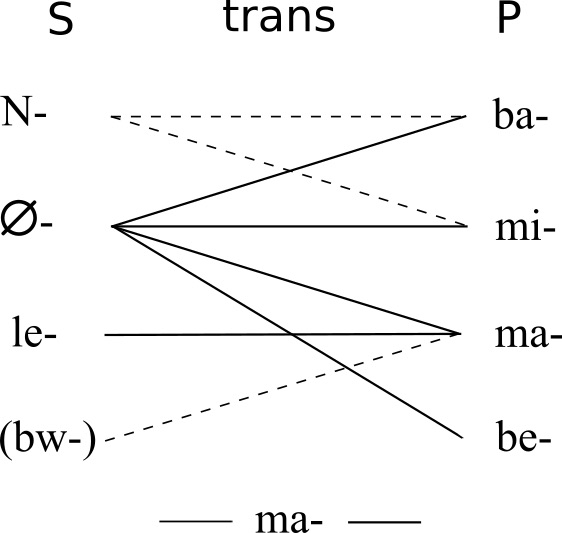
\includegraphics[width=.4\textwidth]{figures/Gyeli-NC-system.jpg}
\caption{Noun prefix class pairings}
\label{Fig:NCs}
\end{figure}

\noindent Although the number of major noun prefix class pairings, including the transnumeral category, and the number of major genders is equal, the patterns in which noun prefix classes and agreement classes pair are substantially different. (For comparison, see \sectref{sec:genders}.)\footnote{For both noun and agreement classes, the decision on what constitutes a major versus a minor class is based on frequency. I consider all classes as major if they represent 4\% or more nouns of the database.}

\tabref{Tab:NCpair} shows the frequency of each noun prefix class pairing. Just as noun prefix classes by themselves differ significantly in size, so do their pairings. For instance, while the smaller noun prefix class pairings such as ``$\emptyset$''-/``ma''- or the transnumeral noun prefix class ``ma''- each cover only a little more than 4\%  of the noun database, the largest noun prefix class pairing, ``$\emptyset$''-/``be''-, constitutes a third of all noun prefix class pairings.
In addition to the 37 nouns in the transnumeral ``ma''-class, there are another 35 nouns that lack a singular or plural form. These are subsumed under ``minor transnumerals''. Their distribution is further specified in \tabref{Tab:genderno}.
  \clearpage


\begin{table}
\begin{tabular}{l rr}
 \lsptoprule
Noun prefix class pairing	&  \multicolumn{2}{r}{Frequency} \\  \midrule
N-/ba 			& 23 & 2.6\% \\
N-/mi- 			&   3 & 0.3\% \\
$\emptyset$/ba- 	& 139  & 15.9\% \\
$\emptyset$/mi- 	&   165 & 18.9\% \\
$\emptyset$/ma- 	&   40  & 4.6\% \\
$\emptyset$/be- 	&   296 & 33.8\% \\
le-/ma- 			&   136 & 15.6\% \\
(bw-/ma-) 		&    1    & 0.1\% \\
ma- 				&  37   & 4.2\% \\
(Minor transnumerals) & 35  & 4\% \\  \midrule
Total 			& 875 & \\  \lspbottomrule
\end{tabular}
\caption{Frequency of noun prefix class pairings}
\label{Tab:NCpair}
\end{table}





\subsection{The Gyeli gender system}
\label{sec:genders}

The nine agreement classes in Gyeli form six major genders, as illustrated in \figref{Fig:Gender}. The major genders are pairings of agreement classes 1/2, 3/4, 5/6, 7/8, and 9/6. Further, the language has one major transnumeral gender, which only involves agreement class 6 without a singular-plural pairing.\footnote{The lack of a counterpart in the singular or plural ties in with mass and/or abstract nouns and countability and is discussed in \sectref{sec:mass}.}
There are other transnumeral nouns outside of gender 6 which do not have a counterpart in the singular or plural. Based on their low frequency, however, they are discussed as inquorate genders in \sectref{sec:MinGen}, together with other low-frequency genders such as 7/6 or 3/6.

\begin{figure}
% 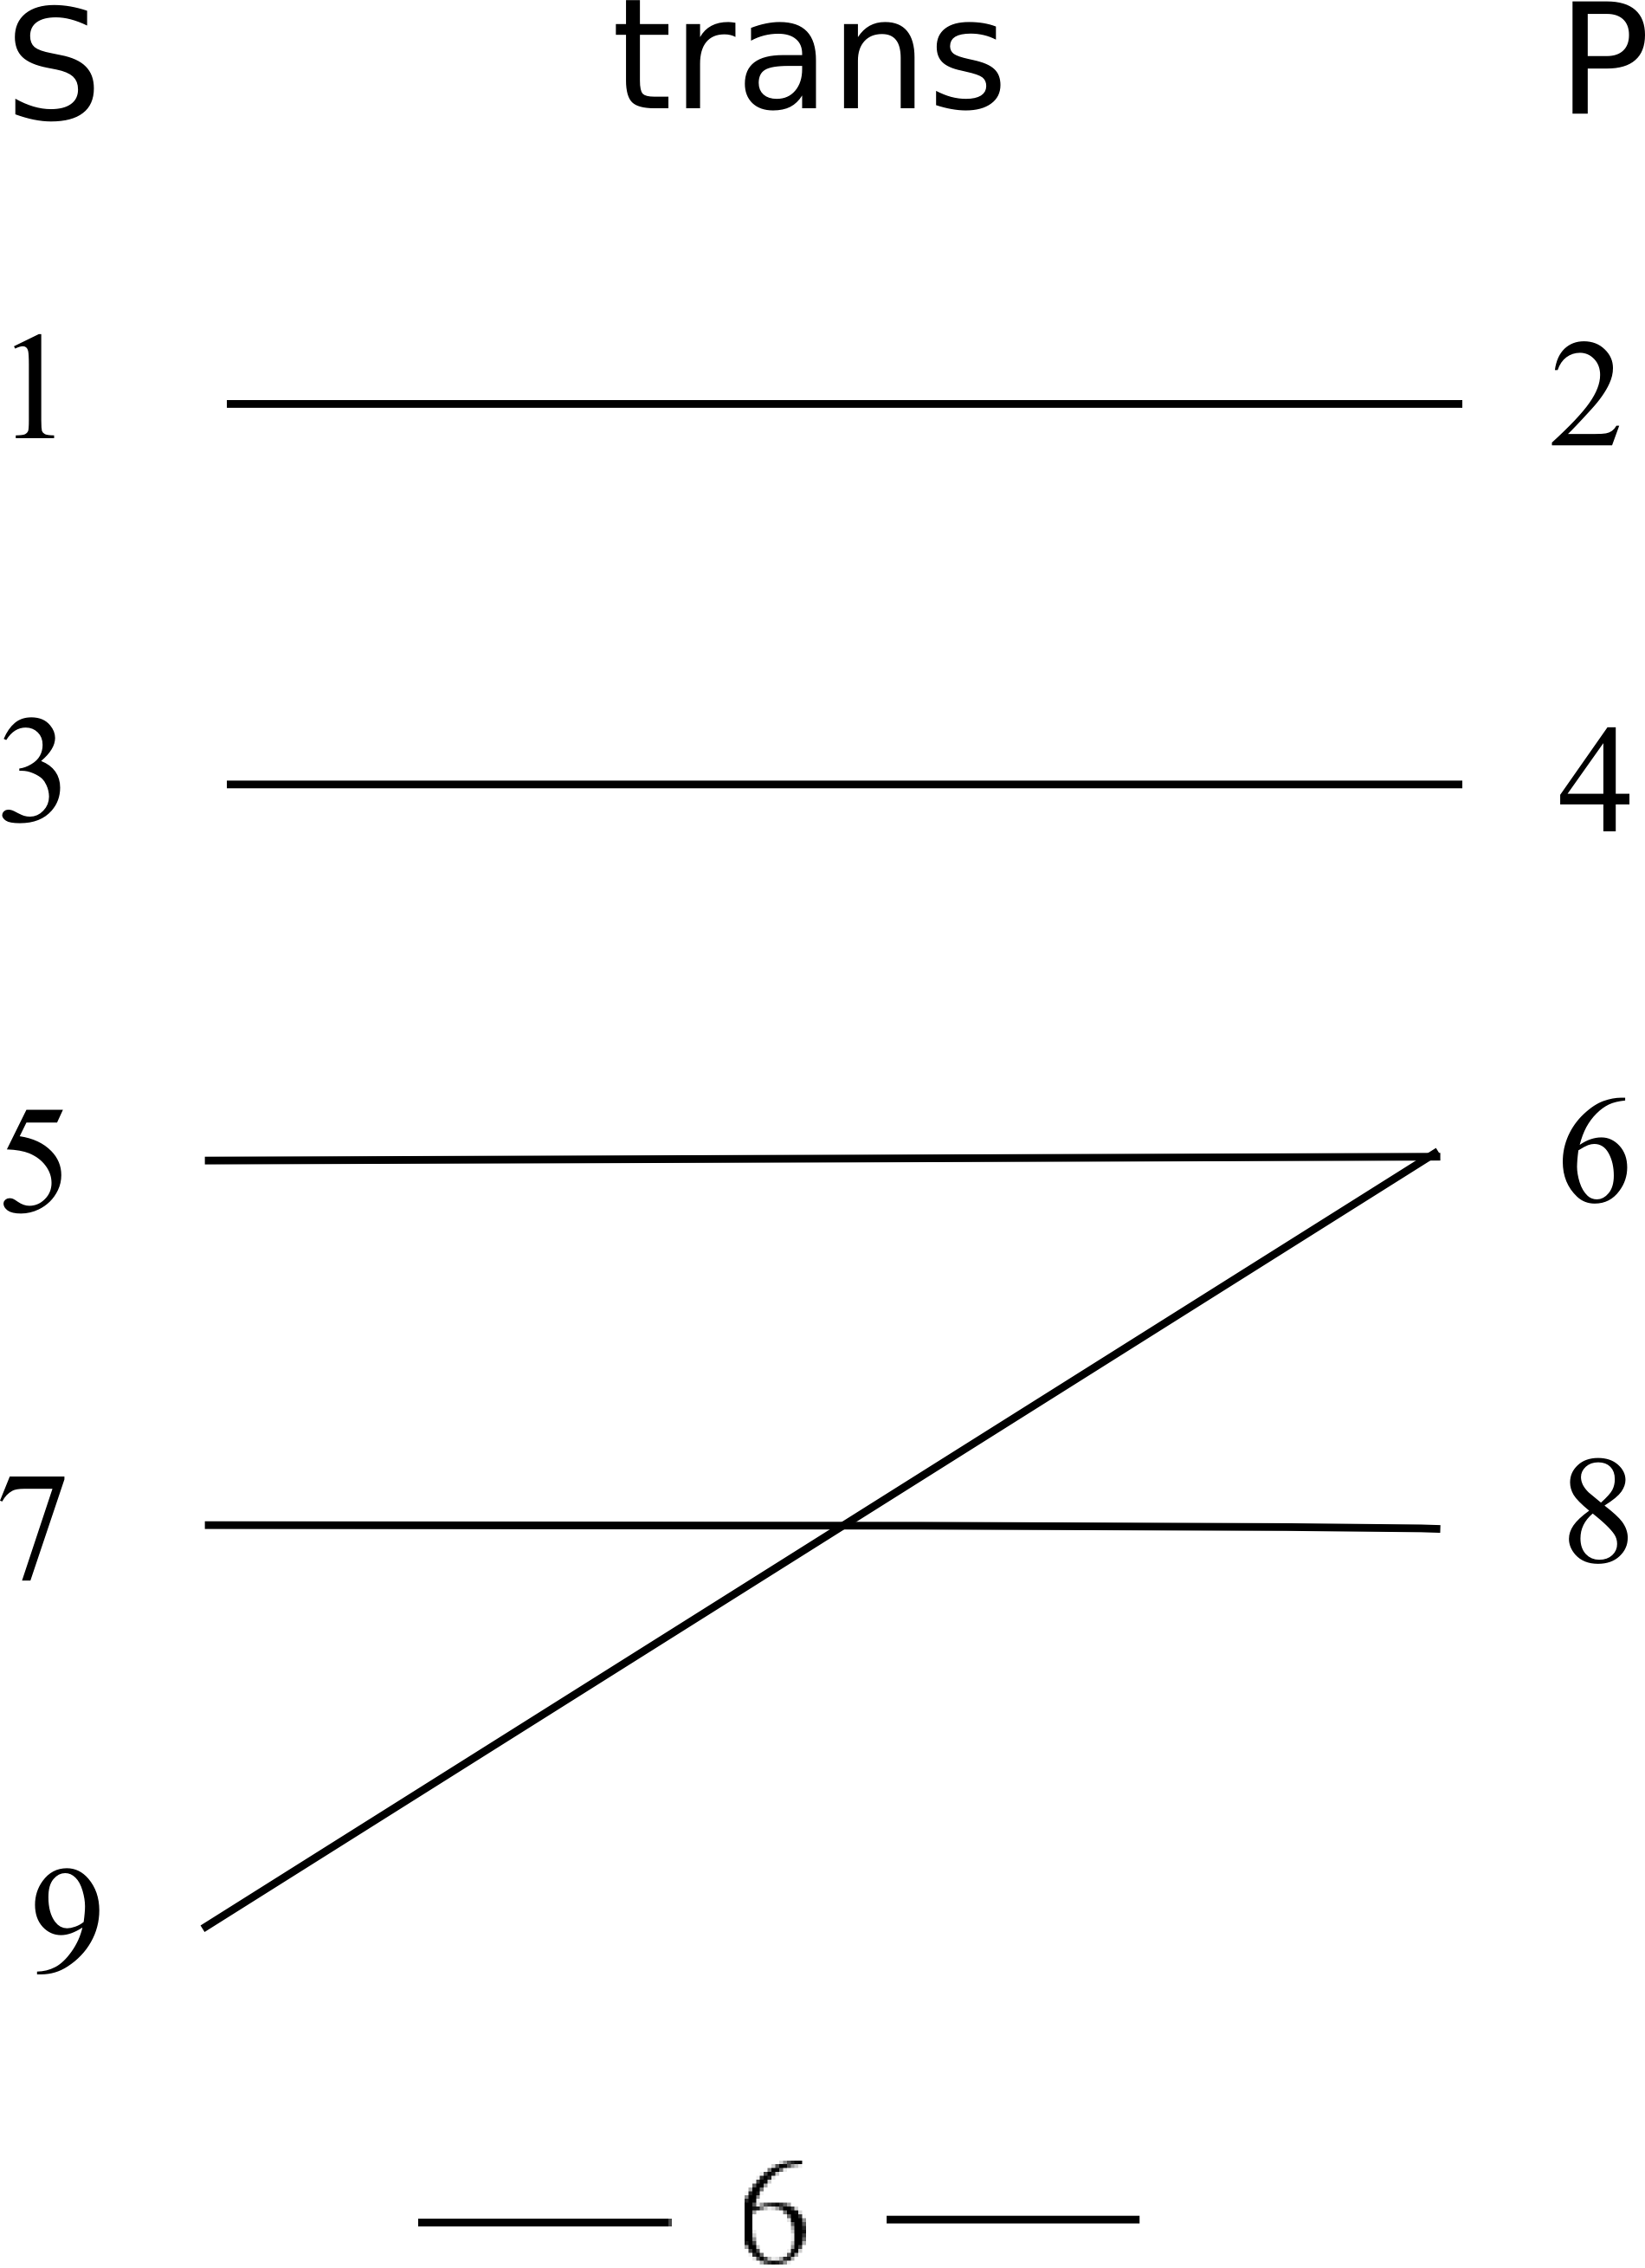
\includegraphics[width=.4\textwidth]{figures/Gyeli-gender-system.png}
\begin{tikzpicture}
\node(1){1};
\node(3)[below=5mm of 1]{3};
\node(5)[below=5mm of 3]{5};
\node(7)[below=5mm of 5]{7};
\node(9)[below=5mm of 7]{9};
%
\node(2)[right=4cm of 1]{2};
\node(4)[below=5mm of 2]{4};
\node(6)[below=5mm of 4]{6};
\node(8)[below=5mm of 6]{8};
%
\node(S)[above=3mm of 1]{\large\scshape sg};
\node(P)[above=3mm of 2]{\large\scshape pl};
\node(trans)[right=1cm of S]{\large\scshape trans};
\node(6b)[below=5mm of 9,xshift=23mm]{6};
\node(6b1)[left=of 6b]{};
\node(6b2)[right=of 6b]{};
%
\draw (1)--(2);
\draw (3)--(4);
\draw (5)--(6.west);
\draw (7)--(8);
\draw (9)--(6.west);
\draw (6b1)--(6b);
\draw (6b)--(6b2);
\end{tikzpicture}
\caption{Major genders in Gyeli}
\label{Fig:Gender}
\end{figure}


\citet{wals-32} states that the way nouns are assigned to a gender can be either strictly semantic, predominantly semantic, or based on a combination of semantic and formal criteria. In strictly semantic systems, the affiliation of a noun to a gender can be deduced from its meaning. Predominantly semantic systems have more complex assignment rules and therefore the semantic grounds on which affiliation to a gender is based are less clear. \citet[2]{wals-32} notes that in these languages, ``for at least some nouns there is no longer a principle for assignment which is still ``live'' for current speakers''.  
Formal criteria, both phonological and morphological, can account for noun assignment to a gender in some languages, but there are no gender assignment systems that are entirely form-based.  Instead, formal criteria occur in combination with semantic assignment criteria \citep[13]{wals-32}.


For Bantu languages, \citet[map 32]{wals-32} states  that gender is typically assigned on both semantic and morphological grounds.
In Gyeli, semantic affiliation of a noun to a certain gender is often opaque and semantic principles governing gender assignment are much less clear-cut, at least synchronically. One cannot say, for instance, that nouns designating humans belong by default to gender 1/2, which is the typical ``human'' gender in Bantu languages. It is true that a large part of gender 1/2 comprises humans, but words for humans are also found in almost all the other genders. The same is true for animals, body parts, tools, plants, and other semantic fields. Not one of them is exclusively found in one gender, but spread across several genders.\footnote{\citet[3]{contini2000}  claims in her cognitive grammar approach to Swahili that ``[n]oun classes [are] semantic in origin but [...] have lost much of their semantic coherence over time''.  In order to verify whether this claim applies to Gyeli as well, much more data would be required which exceeds the limits of this grammar.}

There are, however, some tendencies in the mapping of nouns from different semantic fields onto the various genders, which are based on frequency. Thus, even though human nouns are found in many genders, they are most frequently and thus most typically found in gender 1/2.  Most liquids are uncountable and are found in the transnumeral gender 6. 
Another tendency in gender assignment concerns loanwords, which are most frequently found in gender 1/2 and less often in gender 7/8.


The various genders differ in size, i.e.\ the number of members they have.
\tabref{Tab:genderno} shows the distribution of the 875 lexemes in the nominal database across different genders, distinguishing major and inquorate genders.


\begin{table}
\begin{tabular}{ll rr}
 \lsptoprule
 & Gender &  \multicolumn{2}{l}{Frequency}  \\ 
 \midrule
 \multirow{6}{*}{{Major genders}} & 1/2 & 162 & 18.5\%  \\
 & 3/4  & 165 & 18.9\% \\
 & 5/6  & 136 & 15.5\%   \\
& 7/8   & 270 & 30.9\% \\
& 9/6   & 40  & 4.6\% \\
 & 6 &  37 & 4.3\% \\
 \midrule % minor genders
 \multirow{11}{*}{{Inquorate genders}} &  7/6  & 24  & 2.7\% \\
 & 7   & 13  & 1.5\% \\
 & 8   & 12  & 1.4\% \\
 & 9   & 3  & 0.3\% \\
 & 3/6  & 2  & 0.2\% \\
 & 8/6   &  2 & 0.2\% \\
& 8/8   & 2 & 0.2\% \\
% \midrule         % transnumeral genders
&  4   & 2  & 0.2\% \\
 & 1   & 2  & 0.2\% \\
 & 3   & 2  & 0.2\% \\
 & 5   & 1  & 0.1\% \\
 \midrule
Total & &  875 & \\
 \lspbottomrule
\end{tabular}
\caption{Frequency of genders}
\label{Tab:genderno}
\end{table}

The largest gender is gender 7/8 with over 30\% of the nouns in the database, followed by genders 3/4 and 1/2. The major genders with the least members are genders 9/6 and the transnumeral gender 6. The pairing of agreement classes 7 and 6  constitutes the largest inquorate gender, representing 2.7\% of the lexemes in the noun database. Other inquorate genders with more than 1\% are the transnumeral genders 7 and 8 while all other exceptional patterns are only represented between one and three times in the noun database.

In the following, I discuss each gender in turn, including the semantic fields of the nouns in a given gender and examples of these. In order to determine the semantic field of a noun, I coded nominal entries according to the database \citet{haspelmath2009} use in their world loanword typology. The authors distinguish 24 categories differentiating, for instance, ``the physical world'', ``kinship'', ``animals'', ``body'', ``food and drink'', ``clothing'', ``house'', ``vegetation'', ``technology'', and ``time''.\footnote{For a complete list of all categories and their affiliated lexemes as well as their coding, see \citet[22-34]{haspelmath2009}.}

\largerpage
\subsubsection{Gender 1/2} 
\label{sec:1/2}

Gender 1/2  is a fairly large gender with regard to the number of nouns that are assigned to it with 162 members out of 875 nominal lexical entries. This gender is traditionally referred to as the ``human'' gender in Bantu studies, but seems to have been extended to an ``animate'' gender in Gyeli.  Only about 30\% of the nouns do refer to humans (if one excludes agentive deverbal nouns). Most of these human nouns designate kinship and a few social relations, as shown in \REF{1/2kin} and \REF{1/2soc}. In comparison to other genders containing human nouns, however, gender 1/2 contains the vast majority.

\ea\label{1/2kin} Kin relations
\ea sã́/ba-sã́ `father'
\ex nyã̂/ba-nyã̂ `mother'
\ex n-túmbà/ba-túmbà `older male relative'
\ex ntɛ̀mbɔ́/ba-ntɛ̀mbɔ́ `younger sibling'
\ex kálɛ́/ba-kálɛ́ `older sister'
\z
\ex\label{1/2soc} Social relations
\ea sɔ́/ba-sɔ́ `friend'
\ex n-gyɛ̃̂/ba-gyɛ̃̂ `stranger'
\ex kfúmá/ba-kfúmá `chief'
\ex mbúmbù/ba-mbúmbù `person with the same name'
\ex ngã̂ngã̂/ba-ngã̂ngã̂ `healer'
\z
\z

\noindent 39\% of the gender's nouns belong to the semantic field of animals, both bigger and smaller, as illustrated in \REF{1/2animals}.

\ea\label{1/2animals} Animals
\ea tsídí/ba-tsídí `animal, meat'
\ex kímì/ba-kímì `monkey'
\ex nyû/ba-nyû `bee'
\ex fû/ba-fû `fish'
\ex nyúà/ba-nyúà `snake'
\z
\z

\noindent  The remaining 30\% cover a variety of semantic fields such as ``food'', ``clothing'', ``house'', ``vegetation'', or ``modern world''. It is remarkable that at least more than a third of them constitute loanwords that are borrowed especially from English and French as shown in \REF{1/2loan}. They designate most often recently introduced items in the area of clothing, food, and the modern world.

\ea\label{1/2loan} Loanwords
\ea sɔ́tì/ba-sɔ́tì `trousers (<  English: shorts)'
\ex fàrínì/ba-fàrínì `flour (<  French: {\itshape farine})'
\ex mɔ̀nɛ́/ba-mɔ̀nɛ́ `money'
\ex màtèlà/ba-màtèlà `mattress (< French: {\itshape matelas})'
\ex ngóvìnà/ba-ngóvìnà `government'
\z
\z

\noindent Finally, the absence of a semantic field may be remarkable as well. While ``body'' nouns\footnote{The semantic field ``body'' not only contains body parts, but also body functions, health and disease vocabulary, and  terms related to life cycles.} are found with a relatively high percentage in all other genders, they are virtually absent in gender 1/2. So far, I have found only three instances, all of which designate humans that have a health condition, such as {\itshape njímí/ba-njímí} `blind person', {\itshape búɔ̀/ba-búɔ̀} `mute person', and {\itshape nɔ́ɔ́/ba-nɔ́ɔ́} `deaf person'. Body parts, however, are completely absent in this gender.

\subsubsection{Gender 3/4} 
\label{sec:3/4}

Gender 3/4 is about the same size as gender 1/2 with 165 members out of 875 nominal lexemes. In terms of the meaning of its nouns, the gender is more diverse concerning the semantic fields it covers. The biggest part of its vocabulary belongs to the field of body parts with about 27\%, examples of which are given in \REF{3/4body}.

\ea\label{3/4body} Body
\ea nlô/mi-nlô `head'
\ex d-ìsì/m-ìsì `eye'
\ex nyùmbù/mi-nyùmbù `mouth'
\ex mɔ̀/mi-mɔ̀ `stomach'
\ex n-sùnɛ̀/mi-sùnɛ̀ `calf'
\z
\z

\noindent Examples in \REF{3/4world} represent the next biggest semantic field in gender 3/4 with about 14\% of nouns designating objects in the ``physical world''.

\ea\label{3/4world} Physical world
\ea nsá/mi-nsá `shore'
\ex nkìyɔ́/mi-nkìyɔ́ `wave'
\ex mpá/mi-mpá `island'
\ex nsɛ́/mi-nsɛ́ `sand'
\ex nkúdɛ́/mi-nkúdɛ́ `cloud'
\z
\z

\noindent Further, a relatively large part (11\%) of the lexicon in gender 3/4 designates what the Loanword Database labels as ``basic actions/technology'', as exemplified in \REF{3/4tech}.

\ea\label{3/4tech} Technology
\ea ntúmɛ́/mi-ntúmɛ́ `walking stick'
\ex ntúmò/mi-ntúmò `knife'
\ex nkwɛ̌/mi-nkwɛ̌ `basket'
\ex nkúnkúmbɛ́/mi-nkúnkúmbɛ́ `bow'
\ex nkwálá/mi-nkwálá `machete'
\z
\z

\noindent Animals are also represented in this gender with more than 8\%; \REF{3/4animal} gives examples of some of them.

\ea\label{3/4animal} Animals
\ea ntsã̂ntsúgɛ́/mi-ntsã̂ntsúgɛ́ `dragonfly'
\ex nsĩ̂/mi-nsĩ̂ `African linsang'
\ex nkâ/mi-nkâ `colobus monkey'
\ex nkwúlɔ́/mi-nkwúlɔ́ `cricket'
\ex mbúlɔ̀/mi-mbúlɔ̀ `locust'
\z
\z

\noindent Nevertheless, the remaining 40\% of nouns cover a wide range of semantic fields including ``food'', ``kin'', ``house'', ``vegetation'', ``language'', and ``time'', as illustrated in \REF{3/4other}, just to name a few.

\ea\label{3/4other}  Others
\ea nkwànɔ̀/mi-nkwànɔ̀ `honey'
\ex mbàmbà/mi-mbàmbà `co-wife'
\ex mbɛ̂/mi-mbɛ̂ `door'
\ex mpìngá/mi-mpìngá `cassava'
\ex nlã̂/mi-nlã̂ `story'
\ex mbvû/mi-mbvû `year'
\z
\z


\subsubsection{Gender 5/6}
\label{sec:5/6}

Gender 5/6 is slightly smaller than genders 3/4 and 1/2 with 136 members. Like gender 3/4, it contains many body parts \REF{5/6body}, namely 33\%. The assignment of a body part noun to gender 3/4 or 5/6 seems to be arbitrary since no semantic or form-based pattern is obviously discernible.

\ea\label{5/6body} Body
\ea d-úú/m-úú `nose'
\ex le-lɔ̂/ma-lɔ̂ `ear'
\ex le-nkɛ́dɛ́/ma-nkɛ́dɛ́ `hip'
\ex le-tɔ́lɛ̀/ma-tɔ́lɛ̀ `navel'
\ex le-bɛ́lɛ̀/ma-bɛ́lɛ̀ `breast'
\z
\z

\noindent Further, gender 5/6 contains roughly 19\% animal nouns. Judging from  examples such as in \REF{5/6animals}, size or habitat of an animal seem not to determine its gender affiliation since quite a range of different animals are found in this gender.

\ea\label{5/6animals} Animals
\ea le-bóndó/ma-bóndó `frog'
\ex d-á/m-á `crab'
\ex le-bwǐ/ma-bwǐ `hyena'
\ex le-kénó/ma-kénó `duiker'
\ex j-áwɛ̀/m-áwɛ̀ `goliath frog'
\z
\z

\noindent Humans are also found in this gender which, according to the Loanword Database, are spread over various semantic fields such as ``kin'', ``social relations'', ``religion'', and ``body'' (for the ``defective'' or sick humans), as exemplified in \REF{5/6hum}. Taking these different categories together, human nouns make up 9\% of gender 5/6.

\ea\label{5/6hum} Humans
\ea le-wǎ/ma-wǎ `twin'
\ex le-wányɛ̀/ma-wányɛ̀ `young man'
\ex le-kàgà/ma-kàgà `bewitched woman'
\ex le-tɔ́ndí/ma-tɔ́ndí `lover'
\ex le-bùɔ́/ma-bùɔ́ `cripple'
\z
\z

\noindent Further, gender 5/6 includes a small number of nouns belonging to the domain of ``house'' and the ``physical world'' with about 7\% each and exemplified in \REF{5/6house} and \REF{5/6world} respectively.

\ea\label{5/6house} House
\ea le-wùdɛ̀/ma-wùdɛ̀ `cooking stone'
\ex d-ù/m-ù `oven'
\ex d-ɛ́ndɛ̀/m-ɛ́ndɛ̀ `courtyard'
\ex d-úgó/m-úgó `toilet'
\ex le-yímbálî/ma-yímbálî `entrance' 
\z
\ex\label{5/6world} Physical world
\ea le-nángá/ma-nángá `star'
\ex le-bàdà/ma-bàdà `ground'
\ex le-kɔ́/ma-kɔ́ `stone'
\ex le-lɔ̀ɔ́/ma-lɔ̀ɔ́ `dew'
\ex le-tɔ́/ma-tɔ́ `drop'
\z
\z

\noindent The remaining quarter of gender 5/6 nouns is spread across semantic fields such as ``vegetation'', ``technology'', ``quantity'', ``time'', ``language'', and ``hunting''. \REF{5/6other} gives a few examples.

\ea\label{5/6other} Other
\ea le-lɛ́ndɛ́/ma-lɛ́ndɛ́ `palm tree'
\ex le-kúndí/ma-kúndí `mat'
\ex le-wúmɔ̀/ma-wúmɔ̀ `ten'
\ex le-wùlá/ma-wùlá `hour, time'
\ex le-kɛ́lɛ́/ma-kɛ́lɛ́ `language'
\ex le-lámbɔ̀/ma-lámbɔ̀ `trap'
\z
\z

\noindent Finally, gender 5/6 contains a number of deverbal nouns which are discussed in \sectref{sec:NOM}.


\subsubsection{Gender 7/8}
\label{sec:7/8}

Gender 7/8a is the largest gender in terms of its affiliated nouns with 270 members. ``Body'' \REF{7/8body} and ``animal'' \REF{7/8animals} nouns constitute the majority with both around 20\%.

\ea\label{7/8body} Body
\ea vìnɔ́/be-vìnɔ́ `finger'
\ex dò/be-dò `thigh'
\ex sɛ́/be-sɛ́ `liver'
\ex kúdɛ́/be-kúdɛ́ `skin'
\ex gímù/be-gímù `tongue'
\z
\ex\label{7/8animals} Animals
\ea nɔ̀nɛ́/be-nɔ̀nɛ́ `bird'
\ex tàwɔ̀/be-tàwɔ̀ `goat'
\ex mgbɛ̀mgbɛ̀mɛ̀/be-mgbɛ̀mgbɛ̀mɛ̀ `lion'
\ex sɛ́'ɛ̀/be-sɛ́'ɛ̀ `baboon'
\ex síngì/be-síngì `cat'
\z
\z

\noindent Around 10\% each is taken up by clothing vocabulary as in \REF{7/8cloth} and ``food'' terms as exemplified in \REF{7/8food}.

\ea\label{7/8cloth} Clothes
\ea zíngɔ́/be-zíngɔ́ `short dress'
\ex túnɛ̀/be-túnɛ̀ `scarf for carrying babies'
\ex kàbà/be-kàbà `long dress'
\ex tsílì/be-tsílì `long skirt'
\ex póòlì/be-póòlì `hat'
\z
\ex\label{7/8food} Food
\ea kálá/be-kálá `spice'
\ex kwàndɔ̀/be-kwàndɔ̀ `plantain'
\ex dísì/be-dísì `bowl'
\ex ngùɔ́/be-ngùɔ́ `sugar cane'
\ex búɔ̀/be-búɔ̀ `mortar'
\z
\z

\noindent Another semantic field that is represented in gender 7/8 is ``vegetation'' as in \REF{7/8vege}, however, only with around 6\%.

\ea\label{7/8vege} Vegetation
\ea mpànyè/be-mpànyè `bamboo'
\ex lé/be-lé `tree'
\ex làwɔ́/be-làwɔ́ `branch'
\ex dùwá/be-dùwá `thorn'
\ex kókó/be-kókó `mushroom'
\z
\z

\noindent As in other genders as well, there is a proportion of nouns that belongs to a wide diversity of semantic fields. In gender 7/8, around a third of its member nouns constitute such a semantic diversity. Nouns of semantic fields that are represented with less than 5\% cover semantic domains such as (in decreasing frequency) ``language'', ``physical world'', ``technology'', ``house'', ``hunting'', ``time'', ``social/political relations'', ``spatial relations'', and more. An example of each is provided in \REF{7/8other}.

\ea\label{7/8other} Other
\ea bã̂/be-bã̂ `word'
\ex nkúdɛ́/be-nkúdɛ́ `fog'
\ex tṹũ̀/be-tṹũ̀ `axe'
\ex pìmáá/be-pìmáá `wall'
\ex bwímɔ̀/be-bwímɔ̀ `net hunt'
\ex mɛ́nɔ́/be-mɛ́nɔ́ `day'
\ex túmbɔ́/be-túmbɔ́ `country'
\ex dyá/be-dyá `distance'
\z
\z

\noindent Finally, gender 7/8 also has a few loanwords. This is remarkable because usually loanwords are found in gender 1/2. Gender 7/8 seems to be the only other gender that also takes a few borrowed nouns, as listed in \REF{7/8loan}. Compared to gender 1/2, loanwords are, however, much less numerous in gender 7/8.

\ea\label{7/8loan} Loanwords
\ea sɔ́bì/be-sɔ́bì `soap'
\ex fùláwà/be-fùláwà `flower'
\ex súbì/be-súbì `soup'
\z
\z

There is no obvious semantic or formal pattern that assigns loanwords to gender 7/8 instead of to the default gender for loanwords, which is gender 1/2.  Formally, for instance, {\itshape sɔ́bì} `soap' (gender 7/8) constitutes a minimal pair with the loanword {\itshape sɔ́tì} `trousers' of gender 1/2. Both nouns belong, according to \citet{haspelmath2009}, semantically to the field of ``clothing and grooming''. Another example concerns trisyllabic nouns which start both with /f/ and have the same tonal pattern L H L: {\itshape fùláwà} `flower' belongs to gender 7/8 while {\itshape fàrínì} `flour' belongs to gender 1/2. Gender 7/8 has about 10\% food vocabulary, so it cannot be the case that {\itshape fàrínì} `flour' is not assigned to this gender because it would not fit in semantically. In return, gender 1/2 has some (although few) nouns designating ``vegetation'', so again it cannot be on semantic grounds that {\itshape fùláwà} `flower' is not assigned to the default loanword gender 1/2. One determining factor could be the donor language. It seems that all loanwords in gender 7/8 have an English origin. So far, I have not come across any French loanwords in this gender. In contrast, loanwords in gender 1/2 may come from both English and French. The question still remains then why some English loan nouns are assigned to gender 7/8, while the majority goes into gender 1/2.

\subsubsection{Gender 9/6}
\label{sec:9/6}

Gender 9/6 is the smallest of the major genders with only 40 members in the database of  875 nominal lexemes. Historically, Gyeli has lost agreement class 10, which agreement class 9 would pair with in most other Bantu languages. Instead, Gyeli class 9 pairs synchronically with class 6. In comparison to inquorate genders (\sectref{sec:MinGen}), gender 9/6 has, however, still a significant number (> 4\%) of members. Even more importantly, agreement class 9 always pairs with agreement class 6, while agreement classes that occur in inquorate genders pair with other classes more often than they do in major genders. 

Semantically, a large part of gender 9/6 nouns (about 29\%) belong to the field of  ``body'' nouns. Examples are given in \REF{9/6body}.


\ea\label{9/6body} Body
\ea nyúlɛ̂/ma-nyúlɛ̂ `body'
\ex mbɔ̀mbɔ́/ma-mbɔ̀mbɔ́ `face'
\ex mbvṹɔ̃̀/ma-mbvṹɔ̃̀ `hair'
\ex tsĩ́/ma-tsĩ́ `neck'
\ex ndzílíkɔ̃̂/ma-ndzílíkɔ̃̂ `elbow'
\z
\z

\noindent Further, a relatively big part (14\%) of gender 9/6 nouns belongs to the semantic field of ``language and speech'' as illustrated in \REF{9/6lang}.

\ea\label{9/6lang} Language
\ea ngɔ̀mɔ̀/ma-ngɔ̀mɔ̀ `little drum (tam tam)'
\ex pɔ́/ma-pɔ́ `news'
\ex tsĩ̂/ma-tsĩ̂ `voice'
\ex mpàálé/ma-mpàálé `message'
\z
\z

\noindent Both the physical world and ``house'' vocabulary is represented with about 9\% each and exemplified in \REF{9/6world} and \REF{9/6house} respectively.

\ea\label{9/6world} Physical world
\ea mbí'ìlì/ma-mbí'ìlì `charcoal'
\ex sí/ma-sí `ground'
\ex pfùdí/ma-pfùdí `mold'
\z
\ex\label{9/6house} House
\ea ndáwɔ̀/ma-ndáwɔ̀ `house'
\ex ntábò/ma-ntábò `washing place'
\ex ngɛ̃̂/ma-ngɛ̃̂ `garden'
\z
\z

\largerpage
\noindent The remaining 40\% of nouns belong to semantic fields such as ``food'', ``technology'', ``motion'', ``spatial relations'', ``law'', ``religion'', and more. Some examples representing the listed semantic domains are given in \REF{9/6other}.

\ea\label{9/6other} Others
\ea ndzà/ma-ndzà `hunger'
\ex nkábɛ́/ma-nkábɛ́ `paddle'
\ex ndzì/ma-ndzì `path'
\ex nkwàló/ma-nkwàló `edge'
\ex mpìndá/ma-mpìndá `prohibition'
\ex nkwɛ́lɛ̀/ma-nkwɛ́lɛ̀ `witchcraft'
\z
\z

\subsubsection{Gender 6} 
\label{sec:6}

The transnumeral gender 6 is the smallest of the major genders with only 37 members (4.3\% of nouns in the database). Semantically, it mostly includes liquid mass nouns, as exemplified in \REF{0/6a}.

\ea\label{0/6a}
\ea ma-jíwɔ́ `water'
\ex ma-wã̂ `fat'
\ex ma-nyɔ́ɔ̀ `drink, wine'
\ex ma-nyálɛ̀ `urine'
\ex ma-dyúmù `sperm'
\z
\z

\noindent Other instances of nouns in this gender cover deverbal eventive nouns, as shown in \REF{0/6b}.

\ea\label{0/6b}
\ea ma-dìlá `funeral' <  dìlɛ `bury'
\ex ma-dígà `vision' <  dígɛ `watch'
\ex ma-bwálɛ́ `birth' <  bwálɛ `be born'
\z
\z


\subsection{Inquorate genders}
\label{sec:MinGen}

Inquorate genders are those which have so few members (i.e.\ less than 4\% of the nominal lexemes in the database) that I prefer to treat them as exceptions rather than full-fledged genders in order not to artificially inflate the gender system. Inquorate genders in Gyeli contain the same  agreement classes as major genders. Just their pairing is exceptional. For instance, agreement class 7 usually pairs with agreement class 8. In some exceptions, however, agreement class 7 pairs with class 6 and thus does not belong to the same gender as gender 7/8. Instead, it will be called gender 7/6. Inquorate genders in Gyeli are listed in \tabref{Tab:genderno}  and will be discussed in order of decreasing member numbers.

\subsubsubsection*{{\bfseries Gender 7/6}}
The inquorate gender 7/6 has 24 members in the nominal database. It covers widely diverse semantic fields such as ``body'', ``vegetation'', ``social relations'', ``animals'', ``hunting'', and ``possession''. \REF{7/6} provides some examples.


\ea\label{7/6}
\ea bɛ̀/ma-bɛ̀ `shoulder'
\ex ntúà/ma-ntúà `mango'
\ex kwádɔ́/ma-kwádɔ́ `village'
\ex yílì/ma-yílì `viper'
\ex wáádɔ́/ma-wáádɔ́ `net (for hunting)'
\ex mbúlá/ma-mbúlá `debt'
\z
\z

\noindent It is likely that nouns in this minor gender stem from various classes, but they are difficult to trace back since there are no matching Proto-Bantu reconstructions. Only  {\itshape bɛ̀} `shoulder', out of all 7/6 nouns, can be reconstructed as *-{\itshape bègà} according to \citet[154]{guthrie67}, and belonged to gender 5/6 \citep[101]{meeussen67}.
Other nouns such as `debt' or `mango' do not occur in Meeussen's and Guthrie's reconstructions, while  {\itshape kwádɔ́} `village' in Gyeli does not seem to have any relation with the Proto-Bantu reconstructions in \citet[27]{guthrie71}. Likewise, it is then not clear whether the singular class of a noun has switched agreement classes or the plural class or whether both scenarios hold for different nouns. 

\subsubsubsection*{{\bfseries Gender 7}}
The transnumeral gender, which only contains the singular agreement class 7, is represented with 13 members in the noun database. It contains a few abstract nouns that lack a plural, as illustrated in \REF{7/0a}.

\ea\label{7/0a}
\ea sɔ́nì `shame'
\ex mɛ̀vâ `pride'
\ex sɔ̀mɔ̀nɛ̀ `complaint'
\ex ngɔ̀ngɔ̀lɛ̀ `sadness'
\ex pɔ́nɛ́ `truth'
\ex ngwámɛ́ `danger'
\z
\z

\noindent Other nouns that only have a singular form in agreement class 7 are country names, as shown in \REF{7/0b}.

\ea\label{7/0b}
\ea fàlà `France'
\ex ngyàmànɛ̀ `Germany'
\ex ìtálíyɛ̀n `Italy'
\z
\z



\subsubsubsection*{{\bfseries Gender 8}}
There are also 12 nouns in the database which only have a form in agreement class 8, but no singular or plural counterpart. Like with the transnumeral gender 7, they include abstract nouns, as listed in \REF{0/8a}.


\ea\label{0/8a}
\ea be-bɛ̃̂ɛ̃̀ `beauty'
\ex be-síyá `imitation'
\ex be-jíì `anger'
\ex be-kílì  `attention, cunning'
\z
\z

\noindent Other nouns of this gender are inherently singular (e.g.\ as a mass noun or a singular occurrence in the world) and lack a plural form, as it is the case with the examples in \REF{0/8b}.

\ea\label{0/8b}
\ea vìyɔ́ `fire'
\ex vísɔ́ `sun'
\z
\z



\subsubsubsection*{{\bfseries Gender 9}}
Agreement class 9 also constitutes a transnumeral gender with three members. They are listed in \REF{0/9}.


\ea\label{0/9}
\ea ngwɛ́lɛ̀ `witchcraft'
\ex mpà'à `vapor, fog'
\ex bvúbvù `multitude'
\z
\z

\subsubsubsection*{{\bfseries Gender 3/6}}
Many exceptional agreement class pairings only occur a couple of times in the database. This is the case with the pairing of agreement classes 3 and 6. The only two examples that I found are shown in \REF{3/6}.


\ea\label{3/6}
\ea m-bɔ́/mà-bɔ́ `arm'
\ex n-ákɔ́/m-ákɔ́ `earwax'
\z
\z


\noindent This lexeme -{\itshape bɔ́} `arm' may be reconstructed to Proto-Bantu *{\itshape -bóko} `arm' which belonged to gender 15/6 according to \citet[102]{meeussen67}.\footnote{Other nouns that \citet[102]{meeussen67} classifies as gender 15/6 nouns, such as `leg', `knee',  or `ear', do not have any reflexes in synchronic Gyeli. Since many of them constitute body parts, this is, however, not surprising. \citet{wilkins96}, for instance, shows that especially body parts, or ``parts of a person'' terminology, as he labels it, are subject to semantic change that follows cross-linguistically natural tendencies. Therefore, synchronic noun stems of body parts may have an entirely different shape than the reconstructed Proto-Bantu forms. In any case, it is not possible to say that historic class 15 nouns merged systematically with class 3.}


\subsubsubsection*{{\bfseries Gender 8/6}}
Agreement class 8 has a few singular nouns. While the plural nouns of agreement class 8 all belong to noun prefix class ``be'', the singular members of agreement class 8 do not take a prefix.\footnote{There is one exception where a singular agreement class 8 noun takes a prefix of the shape {\itshape bw}-, a remnant of a former class 14. Since this is the only example, however, I do not list ``bw'' as a noun prefix class on its own.}
 Historically, agreement class 8 nouns that do not take a prefix have probably merged from a former class 14 as the root  beginning with {\itshape bw}- or {\itshape b}- suggests. This would also be in line with the plural pairing with class 6 since \citet[100]{meeussen67} points out that class 14 in Proto-Bantu formed its plural with class 6. Pairings of class 8/6 are very rare in Gyeli. I only found two examples which are given in \REF{8/6}.

\ea\label{8/6}
\ea bwã̂/ma-bwã̂ `medicine'
\ex bw-álɛ̀/m-álɛ̀ `canoe'
\z
\z



\subsubsubsection*{{\bfseries Gender 8/8}}
There are two other examples where the singular variant of agreement class 8 pairs with the plural class 8, as shown in \REF{8/8}. Although the agreement targets of this gender always have the agreement pattern of class 8, I do not view this gender as transnumeral. The reason for this is that there are two distinct noun forms for singular and plural. In this, they differ from transnumeral genders, such as gender 6, which has no singular/plural opposition in its nominal forms. 

\ea\label{8/8}
\ea bvùlɛ́/be-bvùlɛ́ `night'
\ex bírɛ̀lɛ̀/be-bírɛ̀lɛ̀ `smoke'
\z
\z

\subsubsubsection*{{\bfseries Other exceptional transnumeral genders}}
Except for agreement class 2, all agreement classes show instances where they lack either a singular or plural counterpart. For classes 1, 3, 4, and 5, this is very rare with only one or two examples each. \REF{0/4} shows the two examples found for agreement class 4.


\ea\label{0/4}
\ea mi-ngyɛ̌ `hunting rats (digging out their dens)'
\ex my-ɛ́ `fur'
\z
\z

\noindent Instances where agreement class 1 does not have a plural form concern proper names of countries/continents that are inherently singular, as shown in \REF{1/0}.

\ea\label{1/0}
\ea kàmɛ̀rún `Cameroon'
\ex àfríkà `Africa'
\z
\z

\noindent There are also two examples of agreement class 3 nouns that do not take a plural form in class 4. These are listed in \REF{3/0}.

\ea\label{3/0}
\ea bíwɔ̀ `bad luck'
\ex mbvú `white/grey hair'
\z
\z

\noindent Agreement class 5 only has one member that lacks a plural counterpart, as shown in \REF{5/0}.

\ea\label{5/0}
 dyúwɔ̀ `sky'
\z


\section{Distributive numerals with reduplication} 
\label{sec:Distr}
\sectionmark{Distributive numerals}

Distributives are series of reduplicated numerals. They serve the purpose of disambiguating sentences, such as in \REF{Distr}, which can have either a collective or a distributive reading.

\ea\label{Distr}
 Finn and Riley ate two apples.
\z

\noindent In the collective reading, two apples altogether were shared between Finn and Riley whereas in a distributive interpretation, Finn ate two apples and Riley ate two apples. In English, such sentences can be disambiguated by the use of `each': `Finn and Riley ate two apples each.'

Some languages systematically disambiguate such cases. For those languages, the most common means is reduplication of numerals. \citet{gil13} explains this common strategy by its iconic motivation. According to him, copies of the numeral correspond to multiple sets of entities.

Gyeli also uses the reduplication strategy in order to express distributive numerals. Although reduplication is a common strategy for distributive expression in the languages of the world, \citet{rubino13} states that, ``[t]he phonological nature of the reduplicated material varies from language to language and construction to construction''.   \citet[118]{borchardt11} shows that the Benue-Congo language Ikaan, for instance, uses several types of reduplication in order to express distributives. These range from full reduplications including the agreement markers to full root reduplications excluding agreement markers and partial root reduplications. 

In Gyeli, distributive numerals only display one kind of reduplication, namely full reduplication. The numeral, based on its cardinal form, is entirely copied, including its agreement prefixes, if required, and tones, as shown in \REF{nut}.

\ea\label{nut}
  \glll   bwánɔ̀ bà dé mímbàngá {\bfseries mímbáà} {\bfseries mímbáà}\\
         b-wánɔ̀ ba dè-H mí-mbàngá mí-mbáà mí-mbáà\\
                ba2-child 2.{\PST}1 eat-{\R} mi4-nut 4-two 4-two \\
    \trans `The children ate two nuts each.'
\z

\noindent Just like cardinal numerals (\sectref{sec:ModNUM}), distributive numerals agree with the head noun in its agreement class if the specific numeral takes an agreement marker. The distributives that take agreement markers are exactly the same as the cardinals that do, namely `2' through `5'. For those modifier numerals that do not take any agreement prefixes (`6' through `9'), they are entirely reduplicated, just without prefixes. Nominal nouns as well as complex numerals involving noun phrases and/or coordination are also fully reduplicated as one would expect from their cardinal form. \tabref{tab:Distributives} lists Gyeli distributives using the noun {\itshape mbàngá} `nut' of gender 3/4 as an example.

\begin{table}
\fittable{\begin{tabular}{lll}
 \lsptoprule
\multicolumn{2}{l}{Examples of distributive numerals}  & Gloss \\
  \midrule
{\itshape mbàngá} & {\itshape mvúdũ̂ mvúdũ̂} & `one nut each' \\
{\itshape mi-mbàngá} & {\itshape mí-mbáà mí-mbáà} & `two nuts each'\\
{\itshape mi-mbàngá} & {\itshape mí-nláálɛ̀ mí-nláálɛ̀} & `three nuts each' \\
{\itshape mi-mbàngá} & {\itshape mí-nã̂ mí-nã̂} & `four nuts each' \\
{\itshape mi-mbàngá} & {\itshape mí-ntánɛ̀ mí-ntánɛ̀} & `five nuts each' \\
{\itshape mi-mbàngá} & {\itshape ntùɔ́ ntùɔ́} & `six nuts each' \\
{\itshape mi-mbàngá} & {\itshape mpúɛ̀rɛ́ mpúɛ̀rɛ́} & `seven nuts each' \\
{\itshape mi-mbàngá} & {\itshape lɔ̀mbì lɔ̀mbì} & `eight nuts each' \\
{\itshape mi-mbàngá} & {\itshape rèbvùá rèbvùá} & `nine nuts each' \\
{\itshape mi-mbàngá} & {\itshape le-wúmɔ̀ le-wúmɔ̀} & `ten nuts each' \\
{\itshape mi-mbàngá} & {\itshape le-wúmɔ̀ ná mí-báà le-wúmɔ̀ ná mí-báà} & `twelve nuts each' \\
{\itshape mi-mbàngá} & {\itshape ma-wúmɔ̀ má-báà ma-wúmɔ̀ má-báà} & `twenty nuts each' \\
{\itshape mi-mbàngá} & {\itshape bwúyà bwúyà} & `a hundred nuts each' \\
{\itshape mi-mbàngá} & {\itshape tɔ́dyínì tɔ́dyínì} & `a thousand nuts each' \\
  \lspbottomrule
\end{tabular}}
\caption{Distributive numerals}
\label{tab:Distributives}
\end{table}



\section{Distributive construction with {\itshape náà}} 
\label{sec:RedQUANT}

%[Is reduplication the right term here since there is the {\itshape nâ} in between the two nouns?] [???]


In order to express distributivity over individuals, a (countable) noun is iterated while {\itshape náà} is inserted to link the two nouns. {\itshape náà} is only used in this context and formally resembles the adverb {\itshape nâ} `still, again', which, however, has a short vowel instead of a long one.  
The quantified noun can occur both in the singular and in the plural, as shown in \REF{each}. The use of plural nouns, as in \REF{each2}, implies a distribution over a set of entities.

\ea\label{each}
\ea \label{each1}
 \gll  m-ùdì  náà m-ùdì \\
          \textsc{n}1-person by \textsc{n}1-person  \\
    \trans `each person'
\ex \label{each2}
  \gll    b-ùdì  náà b-ùdì \\
             ba2-person by ba2-person \\
    \trans `each (set of) people'
\z
\z

Quantification by nominal iteration in the sense of `each' only works for countable nouns. Thus, neither liquid mass nouns nor granular aggregates in their singular form allow for iterated quantification as shown in \REF{noeach}. Granular aggregates in their plural form, however, can enter such a construction that then gives the reading of `each set of entities of x' as in \REF{noeach3}.

\ea\label{noeach}
\ea[*]{\label{noeach1}
 \glll màjíwɔ́ náà màjíwɔ́\\
 ma-jíwɔ́ náà ma-jíwɔ́ \\
        ma6-water by ma6-water  \\
    \trans `each water'}
\ex[*]{\label{noeach2}
  \glll   ndísì náà ndísì \\  
        ndísì náà ndísì \\
              $\emptyset$3.rice by $\emptyset$3.rice \\
    \trans `each rice'}
\ex \label{noeach3}
  \glll mìndísì náà mìndísì \\
       mi-ndísì náà mi-ndísì \\
              mi4-rice by mi4-rice \\
    \trans `each set of packages of rice'
\z
\z




\section{Attributive constructions}
\label{sec:CONC}

In his comparative study on Bantu attributive constructions, \citet{velde2013} defines a ``canonical'' attributive construction as a dependency relation between two nominal constituents. It is also known as ``associative'' or ``genitive construction'' in the Bantu literature. Since in Gyeli these constructions are, however, not confined to genitive contexts, I prefer to call them ``attributive constructions''.  

\citet{velde2013} describes the canonical attributive construction as \textsc{head} (\textsc{r}1) - \textsc{relator} ({\REL}) - \textsc{dependent} (\textsc{r}2), where the relator (attributive marker) links the head noun (\textsc{r}1) to the dependent noun (\textsc{r}2).
He illustrates this with an example from Kagulu (Bantu G12, Tanzania), cited from \citet[86]{petzell2008} in \REF{const}.

\ea\label{const} Kagulu (Bantu G12)\\
  \gll  m-eji\textsubscript{${\R}1$} g-a\textsubscript{${\REL}$} mu-nyu\textsubscript{${\R}2$}\\
              6-water \textsc{vi}-{\ATT} 3-salt\\
    \trans `salt water'
\z

\citet{velde2013} further points out that Bantu languages are heterogeneous with respect to the way they express attributive possession structurally. There is a huge variation in terms of, for instance, the shape of the attributive marker despite its canonical shape of {\AGR}-{\itshape a}. Also, the dependent constituent, which is typically a  noun, can belong to another part of speech. This is the case for Gyeli. In terms of frequency, the dependent constituent is mostly a noun. It can, however, also belong to the category of adjectives, verbs, or interrogative words. While the part of speech of the dependent constituent may belong to various categories, the head of the construction seems always to be a noun. In the following, I will present the different construction types, organized by the part of speech of the dependent constituent.

\subsection{Noun + noun}
\label{sec:NN}

Noun + noun attributive constructions in Gyeli typically express attributive possession. This core meaning, however, is extended to other semantic properties of a noun, e.g.~quantification (`a lot of cats') and location (`front of the house'). I will discuss the different domains of attributive constructions in turn, starting with the core meaning of possession.

Before turning to the different attributive constructions in Gyeli, however, I will first explore a general formal issue: the optional omission of the attributive marker. The central element of an attributive construction is the linking element, the attributive marker (\sectref{sec:ATT} ), which gives the construction its name. Often, however, the attributive marker can be omitted, while in some cases, it is obligatory. 


\subsubsection{Optional omission of the attributive marker}
\label{sec:CONOM}

 In Gyeli, the attributive marker can in many cases be omitted optionally (which seems to be the default case) as shown in \REF{mino}. In special cases, however, the attributive marker is obligatory, as in \REF{djino}.\footnote{The attributive markers in parentheses are optional while those without brackets cannot be omitted, but must obligatorily appear.}

\ea\label{mino}
  \glll     mínɔ̀ (má) básɔ́ \\
  m-ínɔ̀ má ba-sɔ́ \\
              ma6-name 6:{\ATT}  ba2-friend\\
    \trans `the friends' names'
\z

\ea\label{djino}
  \glll    jínɔ̀ lé sɔ́ \\
          j-ínɔ̀ lé sɔ́ \\
              le5-name 5:{\ATT}  $\emptyset$1.friend\\
    \trans `the friend's name'
\z

\noindent This phenomenon cannot be based on free variation, but must be conditioned by some (set of) rules since speakers are consistent in their judgments of optional omission or obligatory presence of the attributive.

The question is then what conditions are at play in the presence or absence of the attributive marker. It seems that multiple factors determine whether the attributive marker has to appear, including (i) phonological factors where a dependent noun that has a CV- shape noun prefix favors omission of the attributive and (ii) semantic factors concerning the relation between the two nouns. In the following, I will go through a number of possible determining factors and point out to what extent they  influence the occurrence of an attributive marker. I will start out with phonological factors, then move on to morphological, and finally to semantic factors.


The H tone of an attributive marker spreads on to a CV- noun prefix of the dependent noun, as shown in \REF{TON} and discussed in \sectref{sec:HTSr}. One could assume that if the H tone of the attributive marker spreads to the otherwise L tone prefix of the dependent noun, the tonal process might mark the dependency relation and an overt attributive marker is not necessary, as in \REF{TON2}. In contrast, agreement classes that have an L tone attributive marker, where no H tone spreading occurs, might determine the obligatory use of the attributive, as would seem to be the case in \REF{TON1}.

\ea\label{TON}
\ea\label{TON2}
 \glll mìnlô (mí) bátsídí \\
 mi-nlô mí ba-tsídí \\
               mi4-head 4:{\ATT} ba2-animal \\
    \trans `the heads of the animals'
\ex \label{TON1}
  \glll   nlô wà tsídí \\
         nlô wà tsídí \\
               $\emptyset$3.head 3:{\ATT} $\emptyset$1.animal  \\
    \trans `the head of the animal'
\z
\z

This turns out not to be the case, however. \REF{pres} counter-exemplifies the tonal hypothesis because in \REF{pres1}, there is no high tone spreading, but the use of the attributive marker is still optional, while in \REF{pres2} there is high tone spreading, but the use of the attributive marker is still obligatory.

\ea\label{pres}
\ea \label{pres1}
  \glll     mpáà (wà) nlàmbɔ́ \\
        m-páà wà nlàmbɔ́ \\
               \textsc{n}1-president 1:{\ATT} $\emptyset$3.country  \\
    \trans `president of the country'
\ex\label{pres2}
 \glll    bàpáà bá nlàmbɔ́ \\
 ba-páà bá nlàmbɔ́ \\
    ba2-president 2:{\ATT} $\emptyset$3.country \\
    \trans `presidents of the country'
\z
\z

In terms of syllable length, there is a tendency for  monosyllabic dependent nouns to require an attributive marker rather than allowing for its omission, as in \REF{PHO}, compared to disyllabic dependent nouns in \REF{pho}. A bit more than half of the elicited attributive constructions with monosyllabic dependent nouns behave this way.%\footnote{[STATE BASIS OF STATISTICS ???]}


\ea\label{PHO}
\ea \label{PHO1}
  \glll    sɔ́ wà ntí \\
  sɔ́ wà n-tí \\
               $\emptyset$1.friend 1:{\ATT} \textsc{n}1-in.law \\
    \trans `the friend of the in-law'
\ex\label{PHO2}
 \glll    bàsɔ́ bá ntí \\
      ba-sɔ́ bá n-tí \\
               ba2-friend 2:{\ATT} \textsc{n}1-in.law \\
    \trans `the friends of the in-law'
\z
\z


\ea\label{pho}
\ea \label{pho1}
  \glll     sɔ́ (wà) bàtí \\
  sɔ́ wà ba-tí \\
               $\emptyset$1.friend 1:{\ATT} ba2-in.law  \\
    \trans `the friend of the in-laws'
\ex\label{pho2}
 \glll    bàsɔ́ (bá) bátí  \\
 ba-sɔ́ bá ba-tí  \\
               ba2-friend 2:{\ATT} ba2-in.law \\
    \trans `friends of the in-laws'
\z
\z


\noindent There are, however, many exceptions, as in \REF{syll}, where the dependent noun is monosyllabic, but the use of the attributive marker is still optional.

\ea\label{syll}
\ea \label{syll1}
  \glll     ndzí (nyà) nsɛ́ \\
  ndzí nyà nsɛ́ \\
              $\emptyset$9.path 9:{\ATT} $\emptyset$3.sand   \\
    \trans `path of sand'
\ex\label{syll2}
 \glll   jìnɔ́ (lé) ntí   \\
 j-ìnɔ́ lé n-tí   \\
              le5-name 5:{\ATT} \textsc{n}3-in.law \\
    \trans `the name of the in-law'
\z
\z

At the same time, these examples concerning syllable length could also relate to number morphology. Monosyllabic nouns are almost exclusively singular while plural nouns are almost exclusively at least disyllabic. So the question is whether a possible conditioning factor relates to syllable length, number morphology, or agreement class affiliation, as I discuss in the following.

Another factor that could determine the obligatory presence of the attributive marker is the number of the dependent noun. If the dependent noun occurs in the singular, the attributive occurrence is often (more than 50\% of the elicited examples) obligatory as exemplified in \REF{pl1}. In fact, out of all cases where the attributive marker is obligatory, more than 75\% have a singular dependent noun. In contrast, if the dependent noun is plural, as in \REF{pl2}, the use of the attributive marker is mostly optional.


\ea\label{pl}
\ea \label{pl1}
  \glll    ndzí nyà táwɔ̀\\
  ndzí nyà táwɔ̀ \\
               $\emptyset$9.path 9:{\ATT} $\emptyset$7.goat \\
    \trans `path of the goat'
\ex\label{pl2}
 \glll     ndzí (nyà) bètáwɔ̀ \\
   ndzí nyà be-táwɔ̀ \\
               $\emptyset$9.path 9:{\ATT} be8-goat \\
    \trans `path of the goats'
\z
\z

\noindent Again, there are examples, such as in \REF{crab}, where the inverse is the case.

\ea\label{crab}
\ea \label{crab1}
  \glll     jìnɔ́ (lé) dá'á \\
  j-ìnɔ́ lé d-á'á \\
               le5-name 5:{\ATT} le5-crab \\
    \trans `name of the crab'
\ex\label{crab2}
 \glll     jìnɔ́ lé má'á \\
 j-ìnɔ́ lé m-á'á \\
              le5-name 5:{\ATT} ma6-crab \\
    \trans `name of the crabs'
\z
\z

Another hypothesis could be that attributive marker optionality is conditioned by gender or agreement class and depends on the gender or noun prefix class of the head noun  or the dependent noun. This is in fact the case in many closely related languages, as described by \citet{henson2007} for Kol (A832),\footnote{\citet[113]{henson2007}  points out for Kol that ``[f]or most singular nouns, the `basic' associative marker is either zero or a tonal marker''.} by \citet{beavon2006} for Njyem (A84)\footnote{\citet[118]{beavon2006} shows that head nouns of classes 1, 9, and 10 in Njyem occur without ``associative'' markers.} and by \citet{heath2003} for Makaa (A83).\footnote{As in Njyem, head nouns of classes 1, 9, and 10 in Makaa do not occur with an associative marker and are therefore zero-marked  in noun + noun constructions according to \citet[341]{heath2003}.} For Gyeli, however, this does not seem to be the case for either the head or the dependent noun. Changing the noun prefix class of the head noun in \REF{R1} allows both optional omission of the attributive marker, as in \REF{R11}, and obligatory use of the attributive marker, as in \REF{R12}.

\ea\label{R1}
\ea \label{R11}
  \glll   sɔ́ (wà) ngyɛ̃̂ \\
  sɔ́ wà n-gyɛ̃̂ \\
               $\emptyset$1.friend 1:{\ATT} \textsc{n}1-stranger \\
    \trans `friend of the stranger'
\ex\label{R12}
 \glll  ndzí nyà ngyɛ̃̂ \\
 ndzí nyà n-gyɛ̃̂ \\
               $\emptyset$9.path 9:{\ATT} \textsc{n}1-stranger \\
    \trans `path of the stranger'
\z
\z


\noindent The same is true for the dependent noun in \REF{R2}. \REF{R21} shows a case where the attributive can be omitted, while it is obligatory in \REF{R22}.

\ea\label{R2}
\ea \label{R21}
  \glll     sɔ́ (wà) mùdã̂ \\
  sɔ́ wà m-ùdã̂ \\
               $\emptyset$1.friend 1:{\ATT}  \textsc{n}1-woman \\
    \trans `friend of the woman'
\ex\label{R22}
 \glll     sɔ́ wà nkwànò \\
 sɔ́ wà nkwànò \\
               $\emptyset$1.friend 1:{\ATT} $\emptyset$3.honey \\
    \trans `friend of honey' (= somebody who likes honey)
\z
\z

\noindent Attributive marker omission also does not depend on whether the head noun and the dependent noun belong to the same noun prefix class. In \REF{7}, all constituents belong to noun prefix class $\emptyset$ and agreement class 7. In \REF{71x}, the use of the attributive is obligatory, while in \REF{72x}, its use is optional.

\ea\label{7}
\ea \label{71x}
  \glll    vɛ́ɛ̀lá yá yí \\
  vɛ́ɛ̀lá yá yí \\
              $\emptyset$7.decoration 7:{\ATT} $\emptyset$7.wood \\
    \trans `decoration of the wood'
\ex\label{72x}
 \glll vɛ́ɛ̀lá (yá) táwɔ̀ \\ 
 vɛ́ɛ̀lá yá táwɔ̀  \\
             $\emptyset$7.decoration 7:{\ATT} $\emptyset$7.goat   \\
    \trans `decoration of the goat'
\z
\z

There is a  tendency to omit the attributive marker when the dependent noun has a syllabic noun prefix as seen, for instance, in \REF{TON2} or \REF{pho1}. This is true for more than 80\% of the elicited attributive construction examples.

Further, at the intersection of phonology and morphology, there is a tendency to avoid successive identical CV morphemes, i.e.~when the attributive marker and the following noun prefix have the same CV pattern as in \REF{double}. In more than 90\% of these cases, speakers prefer to omit the attributive.

\ea\label{double}
\ea \label{double1}
  \glll  bàsɔ́ (bá) bátí \\
  ba-sɔ́ bá ba-tí \\
               ba2-friend 2:{\ATT} ba2-in.law \\
    \trans `the friends of the in-laws'
\ex\label{double2}
 \glll  jìnɔ́ (lé) lékǎ \\
 j-ìnɔ́ lé le-kǎ \\
             le5-name 5:{\ATT} le5-clan   \\
    \trans `the name of the clan'
\z
\z

\noindent Nevertheless, there are again counterexamples, as shown in \REF{fever}.

\ea\label{fever}
  \glll   màdyû má mákǎ \\
  ma-dyû má ma-kǎ \\
               ma6-fever 6:{\ATT} ma6-clan \\
    \trans `the fevers of the clans'
\z

Semantics may also have an impact: it seems that the attributive marker can be omitted when the relation between the two nouns is an identity relation as with names in \REF{name} and colors in \REF{color}.

\ea\label{name}
  \gll     kwádɔ́ (yá) Ngòló \\
               $\emptyset$7.village 7:{\ATT} $\emptyset$3.{\PN} \\
    \trans `the village of Ngolo'
\z

\ea\label{color}
  \gll     nsínó (wá) nábèbè \\
               $\emptyset$3.color 3:{\ATT} red \\
    \trans `the color red'
\z

\noindent Also numeral head nouns are always followed by an optional attributive marker, as shown in \REF{num}.

\ea\label{num}
\ea \label{num1}
  \glll    lèwúmɔ̀ (lé) básɔ́ \\     le-wúmɔ̀ lé ba-sɔ́ \\
               le5-ten 5:{\ATT} ba2-friend  \\
    \trans `ten friends'
\ex\label{num2}
 \glll     bwúyà (yá) básɔ́ \\
 bwúyà yá ba-sɔ́ \\
              $\emptyset$7.hundred 7:{\ATT} ba2-friend \\
    \trans `hundred friends'
\ex\label{num3}
 \glll  tɔ́gyínì (wà) bàsɔ́ \\
 tɔ́gyínì wà ba-sɔ́ \\
              $\emptyset$1.thousand 1:{\ATT} ba2-friend  \\
    \trans `thousand friends'
\z
\z

As explained in \sectref{sec:NNCompound}, the absence of the attributive marker in some noun + noun constructions may be analyzed as  lexicalized compounds. This becomes clear in noun + noun constructions that oppose a variant with an attributive marker to one without, as in  \REF{woman} and \REF{chick}. 

\ea\label{woman}
\ea \label{woman1}
  \glll   sɔ́ wà mùdã̂ \\
  sɔ́ wà m-ùdã̂ \\
               $\emptyset$1.friend 1:{\ATT} \textsc{n}1-woman \\
    \trans `the friend of the woman'
\ex\label{woman2}
 \glll  sɔ́-mùdã̂ \\
       sɔ́-m-ùdã̂ \\
          $\emptyset$1.friend-\textsc{n}1-woman \\
    \trans `the female friend'
\z
\z

\ea\label{chick}
\ea \label{chick1}
  \glll    kfúbɔ̀ wà dyá \\
  kfúbɔ̀ wà dyá \\
              $\emptyset$1.chicken 1:{\ATT} $\emptyset$7.length \\
    \trans `the chicken that is far away'
\ex\label{chick2}
 \glll     kfúbɔ̀-dyá \\
   kfúbɔ̀-dyá \\
            $\emptyset$1.chicken-$\emptyset$7.length   \\
    \trans `the tall chicken'
\z
\z

There is a difference in the semantic relation between the two nouns. The noun + noun constructions that require the attributive marker, as in \REF{woman1} and \REF{chick1}, mark attributive possession. In contrast, their counterparts without the attributive marker, as in \REF{woman2} and \REF{chick2}, denote attribution of a property. In cases where there is a clear meaning difference between two nouns with and without the attributive marker, I analyze the ones without the attributive marker as noun-noun compounds (\sectref{sec:NNCompound}).




A final factor that I consider here concerns prototypicality of use, relating to the most frequent and natural way two nouns are linked. In \REF{country}, for instance, it seems that speakers naturally think of a country usually having only one president. In this case \REF{country1}, the attributive marker can be omitted. If, however, speakers talk about several presidents, as in \REF{country1}, for instance historically successive presidents, this is a more specific usage, which requires the attributive marker.

\ea\label{country}
\ea \label{country1}
  \glll    mpáà (wà) nlàmbɔ́ \\
  m-páà wà nlàmbɔ́ \\
               \textsc{n}1-president 1:{\ATT} $\emptyset$3.country  \\
    \trans `president of the country'
\ex\label{country2}
 \glll     bàpáà bá nlàmbɔ́ \\
 ba-páà bá nlàmbɔ́ \\
               ba2-president 2:{\ATT} $\emptyset$3.country \\
    \trans `presidents of the country'
\z
\z




\subsubsection{Nominal possessives}  
\label{sec:NomPOSS}

Having discussed the optional omission and obligatory presence of the attributive marker in noun + noun constructions, I will, for reasons of simplicity, not indicate anymore whether the attributive is optional or not.  I now turn to semantically different noun + noun constructions. The core meaning of these is that of attributive possession. Examples of possessive noun + noun constructions are given in \REF{possession} with the head noun occurring in different noun prefix classes. The head noun expresses the possessee while the dependent noun expresses the possessor.

\ea\label{possession}
\ea \label{possession1}
  \glll mùdã̂ wà mùdì \\
  m-ùdã̂ wà m-ùdì \\
               \textsc{n}1-woman 1:{\ATT} \textsc{n}1-person  \\
    \trans `the person's wife'
\ex \label{possession2}
  \glll  bùdã̂ bá mùdì \\
  b-ùdã̂ bá m-ùdì \\
               ba2-woman 2:{\ATT} \textsc{n}1-person  \\
    \trans `the person's wives'
\ex \label{possession3}
  \glll dìsí lé mùdì \\
  d-ìsí lé m-ùdì \\
               le5-eye 5:{\ATT} \textsc{n}1-person  \\
    \trans `the person's eye'
\ex \label{possession4}
  \glll     mísì má mùdì \\
  m-ísì má m-ùdì \\
               ma6-eye 6:{\ATT} \textsc{n}1-person  \\
    \trans `the person's eyes'
\z
\z

Gyeli has a split genitive system with two distinct noun + noun linker paradigms: the attributive marker (\sectref{sec:ATT}) and the genitive marker (\sectref{sec:GEN}). The genitive marker is used when the dependent noun is a proper name, while the attributive marker is used everywhere else, as further explained below. 

Interestingly, the language does not have a typical possessive classification system, which most usually distinguishes grammatically between alienable and inalienable possession. \citet{nichols2013} explain that this type of possessive classification is based on properties of the possessee. Typically, inalienable possessions concern kinship relations and body parts, while alienable possessions can be separated from the owner, for instance materials (axe, spear) or food items (mango, bread). According to the WALS map on possessive classification by \citet{nichols2013}, some Niger-Congo languages, such as Gbeya Bossangoa (Central African Republic), Lango and Luganda (Uganda), or Luvale (Angola), have two possessive classes with an alienable/inalienable distinction.

Gyeli does not make a grammatical distinction between alienable and inalienable possession as shown in \REF{INAL}. No matter whether the possessee is a kin \REF{INAL1}, body part \REF{INAL2}, or material possession \REF{INAL3}, the attributive marker always agrees in class with the head noun (possessee).

\ea\label{INAL}
\ea \label{INAL1}
  \glll      nyã̂ {\bfseries wà} mwánɔ̀ \\
  nyã̂ wà m-wánɔ̀ \\
               $\emptyset$1.mother 1:{\ATT} \textsc{n}1-child  \\
    \trans `the child's mother'
\ex \label{INAL2}
  \glll     d-úú {\bfseries lé} mwánɔ̀ \\
  d-úú lé m-wánɔ̀ \\
               le5-nose 5:{\ATT} \textsc{n}1-child  \\
    \trans `the child's nose'
\ex \label{INAL3}
  \glll  nkwálá {\bfseries wá} mwánɔ̀ \\
nkwálá wá m-wánɔ̀\\
               $\emptyset$3.machete 3:{\ATT} \textsc{n}1-child  \\
    \trans `the child's machete'
\z
\z

In Gyeli, the genitive split is conditioned by the type of possessor noun, distinguishing common nouns and proper names. If the possessor is expressed by a proper name, the genitive marker (\sectref{sec:GEN}) is used, as in \REF{splitGEN1}.  If a common noun is used for the possessor instead, as in a parallel construction in \REF{splitGEN2}, the two nouns are linked by an attributive marker.

\ea\label{splitGEN}
\ea \label{splitGEN1}
  \glll      mùdû {\bfseries ngá} Nándtùngù \\
  m-ùdû ngá Nándtùngù \\
\textsc{n}1-man {\GEN} $\emptyset$1.{\PN}  \\
    \trans `Nandtoungou's husband'
\ex \label{splitGEN2}
  \glll  mùdũ̂ {\bfseries wà} mùdã̂\\
  m-ùdũ̂ wà m-ùdã̂ \\
 \textsc{n}1-man 1:{\ATT} \textsc{n}1-woman \\
    \trans `the woman's husband'
\ex \label{splitGEN3}
  \glll màkwámɔ́  {\bfseries má-ngá} Nándtùngù \\
  ma-kwámɔ́ má-ngá Nándtùngù \\
    ma6-bag 6-{\GEN} $\emptyset$1.{\PN}  \\
    \trans `Nandtoungou's bags'
\z
\z

The genitive marker only takes an agreement prefix if the possessee head noun occurs in a plural form, as in \REF{splitGEN3}. Therefore, the genitive marker is conditioned both by the head noun's grammatical number and the dependent noun's status as common or proper noun. The dependent possessor noun determines whether an attributive or a genitive marker is used. The possessee head noun determines number/agreement class marking.


\subsubsection{Properties}  
\label{sec:PROP}

A semantic subcategory of possession are those noun + noun constructions that express a property of the head noun such as `old', `beautiful', or `strong'. These properties are expressed by nouns in Gyeli; examples are given in \REF{nposs}.

\ea\label{nposs}
\ea \label{nposs1}
  \glll     sɔ́ wà ntúlɛ́ \\
  sɔ́ wà ntúlɛ́ \\
               $\emptyset$1.friend 1:{\ATT} $\emptyset$3.oldness  \\
    \trans `old friend'
\ex \label{nposs2}
  \glll bùdã̂ bá bébɛ̃́  \\
  b-ùdã̂ bá be-bɛ̃́  \\
               ba2-woman 2:{\ATT} be8-beauty \\
    \trans `beautiful women'
\ex \label{nposs3}
  \glll    mùdì wà ngvùlɛ́ \\
  m-ùdì wà ngvùlɛ́ \\
               \textsc{n}1-person 1:{\ATT} $\emptyset$9.strength \\
    \trans `strong person'
\z
\z


The property noun + noun constructions differ structurally from nominal possessives in the role of the head noun. While in nominal possessive constructions the head noun is the possessee, in property noun + noun constructions, the head noun is rather the possessor in the unmarked case following a pattern `a man of strength'. The order of head and dependent noun can, however, be reversed while the basic meaning remains the same, as in \REF{tili}.

\ea\label{tili}
\ea \label{tili1}
  \glll  mùdũ̂ wà tílì \\
  m-ùdũ̂ wà tílì \\
               \textsc{n}1-man 1:{\ATT} $\emptyset$7.smallness \\
    \trans `small man'
\ex \label{tili2}
  \glll      tílì yá mùdũ̂ \\
 tílì yá m-ùdũ̂ \\
              $\emptyset$7.smallness 7:{\ATT} \textsc{n}1-man  \\
    \trans `small man/smallness of man'
\z
\z


\REF{tili1} exhibits the unmarked order, which can literally be translated as `man of smallness'. \REF{tili2} is ambiguous because it can  either mean `the smallness of the man', referring to size, or it can refer to the man himself in the sense of `a midget of a man'.
The reversal in the second sense seems  to have pragmatic functions of irony or emphasis. 


\subsubsection{Nominal quantifiers}  
\label{sec:NomQUANT}

Another use of the canonical noun + noun construction concerns expression of quantification. Some quantifiers in Gyeli are nouns and combine with the noun that they quantify as the head of the construction.
Nominal quantifiers include numerals and non-numeral modifiers such as `many', `few', `a certain', `some', and partitive quantifiers such as `half'. Only a few quantifiers in Gyeli make a distinction between countable and non-countable nouns, by restricting the combination of certain quantified nouns with certain quantifier nouns. This is the case, for instance, with {\itshape mwánɔ̀} `little/few', as I will show below.

\subsubsubsection{Numerals} Some monomorphemic numerals in Gyeli constitute nouns. As discussed in \sectref{sec:Enum} on enumeratives, these are the bases of the system, namely {\itshape le-wúmɔ̀} `10' (cl.~5), {\itshape bwúyà} `100' (cl.~7), and {\itshape tɔ́dyínì} `1000' (cl.~1). Being nouns themselves, they do not agree with the noun they quantify. Instead, they can become the head of a noun + noun attributive construction, as shown in \REF{NumNoun}. The two nouns are linked by an attributive marker that can optionally be omitted.

\ea\label{NumNoun}
\ea \label{NumNoun1}
  \glll     lèwúmɔ̀ (lé) básɔ́\\
  le-wúmɔ̀ lé ba-sɔ́\\
                le5-ten 5:{\ATT} ba2-friend \\
    \trans `ten friends'
\ex\label{NumNoun2}
 \glll     bwúyà (yá) básɔ́ \\
 bwúyà yá ba-sɔ́ \\
                $\emptyset$7.hundred 7:{\ATT} ba2-friend \\
    \trans `hundred friends'
\ex\label{NumNoun3}
 \glll     tɔ́dyínì (wà) bàsɔ́ \\
 tɔ́dyínì wà ba-sɔ́ \\
                $\emptyset$1.thousand 1:{\ATT} ba2-friend \\
    \trans `thousand friends'
\z
\z

\noindent The noun + noun construction with an attributive marker is the preferred option to express nominal cardinals, which speakers would judge as ``good Gyeli''. Nevertheless, speakers sometimes adopt the structure of non-nominal cardinals so that the numeral noun follows the quantified noun, as in \REF{NounNum}. The two nouns are then juxtaposed without any attributive marker, thus copying the syntactic structure of noun + modifier numeral noun phrases (\sectref{sec:ModNUM}).

\ea\label{NounNum}
\ea \label{NounNum1}
  \gll     bà-sɔ́ lè-wúmɔ̀\\
                ba2-friend le5-ten \\
    \trans `ten friends'
\ex\label{NounNum2}
 \gll     bà-sɔ́ bwúyà \\
                ba2-friend $\emptyset$7.hundred \\
    \trans `hundred friends'
\ex\label{NounNum3}
 \gll     bà-sɔ́ tɔ́dyínì \\
                ba2-friend $\emptyset$1.thousand \\
    \trans `thousand friends'
\z
\z





\subsubsubsection{{\itshape bvúbvù nyà} `many, lots of'}
Many quantifiers in Gyeli are expressed by a noun + noun attributive construction. In these cases, a quantifying noun serves as the head of the construction, and the quantified noun is linked by an attributive marker that agrees with the head noun, as in \REF{bvubvu}.

\ea\label{bvubvu}
  \glll     bvúbvù nyà bùdì \\
  bvúbvù nyà b-ùdì \\
                $\emptyset$9.multitude 9:{\ATT} ba2-people \\
    \trans `many people'
\z

 {\itshape bvúbvù} `multitude' is used for both countable and non-countable nouns. \REF{bvu} provides examples of quantified nouns that semantically belong to liquids or granular aggregates and that typically are not countable.

\ea\label{bvu}
\ea \label{bvu1}
  \glll     bvúbvù nyà màjíwɔ́ \\
  bvúbvù nyà ma-jíwɔ́ \\
                $\emptyset$9.multitude 9:{\ATT} ma6-water \\
    \trans `lots of water'
\ex\label{bvu2}
 \glll     bvúbvù nyà ndísì  \\
 bvúbvù nyà ndísì  \\
             $\emptyset$9.multitude 9:{\ATT} $\emptyset$3.rice  \\
    \trans `lots of rice'
\ex\label{bvu3}
 \glll   bvúbvù nyà mìnsɛ́   \\
 bvúbvù nyà mi-nsɛ́   \\
             $\emptyset$9.multitude 9:{\ATT} mi4-sand    \\
    \trans `lots of (types of) sand'
\z
\z

Depending on the context, the quantification of mass nouns with {\itshape bvúbvù} `many, lots' can also yield a type interpretation, as in \REF{bvu3}, where it is ambiguous whether the speaker refers to a lot of sand or several types of sand. 

\subsubsubsection{{\itshape mwánɔ̀} `a few, little'}
The counterpart of {\itshape bvúbvù} `many, lots' is {\itshape mwánɔ̀} and its plural form {\itshape bwánɔ̀} `few, little'. The primary lexical meaning of {\itshape mwánɔ̀/bwánɔ̀} is `child/children'. In an attributive construction with a (countable) noun, however, it serves as a quantifier with a meaning of  `a few', as shown in \REF{small1}.

\ea\label{small}
\ea\label{small1}
 \glll bwánɔ̀ bá bákɔ́bɛ̀  \\     
 b-wánɔ̀ bá ba-kɔ́bɛ̀  \\
             ba2-small 2:{\ATT} ba2-cup  \\
    \trans `a few cups'
\ex \label{small2}
  \glll   bwánɔ̀-bákɔ́bɛ̀  \\   
  b-wánɔ̀-ba-kɔ́bɛ̀  \\
    ba2-small-ba2-cup \\
    \trans `small cups'
\z
\z

In contrast, in \REF{small2}, the two nouns form a compound (\sectref{sec:NNCompound}) without the attributive marker and {\itshape bwánɔ̀} `child' expresses the meaning of `small (in size)'. It thus productively serves as a diminutive marker and is, in fact, the only diminutive strategy in the language.

In some cases with countable nouns, however, the attributive marker can be omitted without resulting in a diminutive. Instead, {\itshape mwánɔ̀/bwánɔ̀} serves as a quantifier, as in \REF{ntua}. In these cases, I do not view the attributive-less construction as a compound.

\ea\label{ntua}
\ea \label{ntua1}
  \glll    bwánɔ̀ bá mántúà  \\
  b-wánɔ̀ bá ma-ntúà  \\
    ba2-small 2:{\ATT} ma6-mango \\
    \trans `a few mangoes'
\ex\label{ntua2}
 \glll    bwánɔ̀ mántúà  \\
 b-wánɔ̀ ma-ntúà  \\
             ba2-small ma6-mango  \\
    \trans `a few mangoes'
\z
\z

When asked what they would say for `small mangoes', speakers state that they prefer the use of the adjective {\itshape píyɔ̀} `small' for mangoes, as in \REF{mango}. It is not clear what semantically selects for either {\itshape píyɔ̀} or {\itshape mwánɔ̀} when talking about smallness in size.

\ea\label{mango}
  \glll     màntúà má píyɔ̀ \\
  ma-ntúà má píyɔ̀ \\
                ma6-mango 6:{\ATT} small \\
    \trans `small mangoes'
\z

In contrast to {\itshape bvúbvù} `many, lots', {\itshape mwánɔ̀/bwánɔ̀} `a few, little' is sensitive to countability distinctions. With countable nouns, the plural form {\itshape bwánɔ̀} is obligatorily used, as in \REF{small1}, since the quantified noun can only appear in the plural as the meaning of `few' is inherently plural. For uncountable nouns, however, the singular form {\itshape mwánɔ̀} `little' is used with a singular non-countable noun, as in \REF{little}. 

\ea\label{little}
\ea \label{little1}
  \glll mwánɔ̀ nsɛ́ \\
    m-wánɔ̀ nsɛ́ \\
    \textsc{n}1-small $\emptyset$3.sand\\
    \trans `a little bit of sand'
\ex\label{little2}
 \gll     m-wánɔ̀ ndísì  \\
             \textsc{n}1-small $\emptyset$3.rice  \\
    \trans `a little bit of rice'
\ex[*]{\label{little3}
  \gll   m-wánɔ̀ wà nsɛ́ \\
    \textsc{n}1-small 1:{\ATT} $\emptyset$3.sand\\
    \trans `a little bit of sand'}
\z
\z

While attributive-less constructions with quantified count nouns get a diminutive reading, referring to small size, with non-count nouns, {\itshape mwánɔ̀} does not serve as a diminutive, but as a quantifier. The quantifier construction that requires the attributive marker with count nouns is prohibited with non-count nouns, as shown in \REF{little3}. 


It is possible to use the plural form of uncountable nouns, for those that have a singular/plural pairing, as shown in \REF{PLlittle}.\footnote{Uncountable nouns cannot be quantified with numerals. They differ, however, with respect to the type of gender affiliation and number behavior of the noun. Liquids generally occur in the transnumeral gender 6, while granular aggregates often have a singular/plural pairing.} In these cases, the quantifying noun has to take the plural form as well. Still, in contrast to countable nouns, these constructions never take an attributive marker. The semantic difference between singular and plural forms of mass nouns such as `sand' or `rice' is that the plural form always gets a type-reading, involving several entities of the quantified mass noun. It seems, however, context dependent whether quantification is over the non-count noun (e.g. several entities containing a little bit of sand) or whether quantification is over the amount of entities (e.g. a few entities of sand).

\ea\label{PLlittle}
\ea \label{PLlittle1}
  \glll bwánɔ̀ mìnsɛ́ \\
  b-wánɔ̀ mi-nsɛ́ \\
    ba2-small mi4-sand\\
    \trans `a few entities of sand or entities with a little bit of sand each'
\ex\label{PLlittle2}
 \glll     bwánɔ̀ mìndísì  \\
 b-wánɔ̀ mi-ndísì  \\
    ba2-small mi4-rice  \\
    \trans `a few entities of rice or entities with a little bit of rice each'
\z
\z

In contrast to granular aggregates such as `rice' or `sand', which are uncountable but have a singular and a plural form, liquids are assigned to the transnumeral gender 6 without a singular/plural opposition in the nominal form. They behave morphosyntactically differently because, unlike in \REF{PLlittle}, the transnumeral class 6 does not allow the plural form of the quantifier noun, but requires its singular form, as shown in \REF{littlewater}. This is remarkable since agreement class 6 is by default a plural class with respect to number marking.\footnote{Liquid mass nouns in Gyeli show an interesting difference to Mabi, the closest relative of Gyeli, since in Mabi, `a little bit of water' is expressed with the plural form of the quantifying noun as {\itshape bwá májíwɔ́}.}

\ea\label{littlewater}
\ea \label{littlewater1}
  \gll     m-wánɔ̀ mà-jíwɔ́\\
                \textsc{n}1-small ma6-water \\
    \trans `little water'
\ex[*]{\label{littlewater2}
 \gll     b-wánɔ̀ mà-jíwɔ́  \\
        ba2-small ma6-water  \\
    \trans `little water'}
\z
\z



\subsubsubsection{{\itshape njìmɔ̀ wá} `a certain, some'}
Gyeli does not make any further distinctions in terms of approximate quantities other than `many' and `a few', i.e.\ additional quantifiers such as `a couple' or `several' do not exist. There is a means, however, to express unspecificity of both entity and number: {\itshape njìmɔ̀ wá} `a certain, some' (translated as {\itshape quelconque} in Cameroonian French). Using this quantifier expresses that the entity is not known or specified and also its number or amount remains unspecified. 

{\itshape njìmɔ̀ wá} is used with both singular and plural nouns, as in \REF{ndjimo}, as well as countable and uncountable nouns, as in \REF{ndjimob}.  In contrast to {\itshape mwánɔ̀/bwánɔ̀} `a few, little', which agrees in number with the quantified noun, {\itshape njìmɔ̀ wá} is invariable. 

\ea\label{ndjimo}
\ea \label{ndjimo1}
  \glll   njìmɔ̀ wá mùdì  \\
  njìmɔ̀ wá m-ùdì  \\
 $\emptyset$3.certain 3:{\ATT} \textsc{n}1-person \\
    \trans `a certain person'
\ex\label{ndjimo2}
 \glll    njìmɔ̀ wá  bùdì \\
 njìmɔ̀ wá  b-ùdì \\
$\emptyset$3.certain 3:{\ATT} ba2-people  \\
    \trans `certain people'
\z
\z

\ea\label{ndjimob}
\ea \label{ndjimob1}
  \glll  njìmɔ̀ wá màjíwɔ́ \\
  njìmɔ̀ wá mà-jíwɔ́ \\
        $\emptyset$3.certain 3:{\ATT} ma6-water \\
    \trans `certain water'
\ex\label{ndjimob2}
 \glll    njìmɔ̀ wá mínsɛ́ \\
 njìmɔ̀ wá  mi-nsɛ́ \\
$\emptyset$3.certain 3:{\ATT} mi4-sand  \\
    \trans `certain (types of) sand'
\z
\z


\subsubsubsection{{\itshape bímbú yá} `a quantity of'}
Another quantifier that expresses unspecificity is {\itshape bímbú yá} `a quantity of'. In contrast to {\itshape njìmɔ̀ wá} `a certain', the entity is not unknown, but its number or amount is unspecified.

 Just as the attributive construction with {\itshape bvúbvù} `many, lot', here too,  the quantifying noun serves as head in the noun + noun construction and links the quantified noun with an attributive marker that agrees with the head noun, as in \REF{bimbu}. Also, both countable and uncountable nouns can be used with {\itshape bímbú yá}, i.e.~this quantifier is not sensitive to a mass/count distinction.

\ea\label{bimbu}
\ea \label{bimbu1}
  \glll bímbú yá bùdì \\
  bímbú yá b-ùdì \\
$\emptyset$7.quantity 7:{\ATT} ba2-people \\
\trans `a certain quantity of people (some people)'
\ex\label{bimbu2}
 \glll    bímbú yá màjíwɔ́  \\
 bímbú yá ma-jíwɔ́  \\
$\emptyset$7.quantity 7:{\ATT} ma6-water  \\
    \trans `a certain quantity of water (some water)'
\z
\z

The unspecific noun quantifier can be made more specific in  combination with another quantifier such as {\itshape bvúbvù} `many' and {\itshape mwánɔ̀/bwánɔ̀} `few', as shown in \REF{bimbucomb}. Just like unspecific uses of {\itshape bímbú} `quantity', as in \REF{bimbu}, these constructions are not sensitive to a mass/count distinction, unlike {\itshape mwánɔ̀/bwánɔ̀} `a few'.

\ea\label{bimbucomb}
\ea\label{bimbucomb1}
 \glll   mwánɔ̀  bímbú yá bùdì  \\
 m-wánɔ̀  bímbú yá b-ùdì  \\
 \textsc{n}1-small   $\emptyset$7.quantity 7:{\ATT} ba2-people  \\
    \trans `a small quantity of people'
\ex \label{bimbucomb2}
  \glll    mwánɔ̀ bímbú yá ndísì \\
  m-wánɔ̀ bímbú yá ndísì \\
              \textsc{n}1-small  $\emptyset$7.quantity 7:{\ATT} $\emptyset$3.rice \\
    \trans `a small quantity of rice'
\z
\z

\subsubsubsection{{\itshape tsílɛ̀ yá} `half of'}
Gyeli only has few proportionality quantifiers, one of which is {\itshape tsílɛ̀ yá} `half of'. This quantifying noun is semantically sensitive to a mass/count distinction concerning plural nouns in so far as countable nouns usually come as material entities that can be split in half.
{\itshape tsílɛ̀} `half' refers to material halves rather than half in terms of number, as in \REF{tsile1}. If `half' is meant in a numerical sense, this has to be made explicit with countable nouns by adding {\itshape tã̂ yá} `number of' to the construction, as in \REF{tsile2}.

\ea\label{tsile}
\ea\label{tsile1}
 \glll tsílɛ̀ yá bùdì  \\
 tsílɛ̀ yá b-ùdì  \\
          $\emptyset$7.half 7:{\ATT} ba2-people  \\
    \trans `the half of people (their bodies)'
\ex \label{tsile2}
  \glll    tsílɛ̀ yá tã̂ yá bùdì \\
  tsílɛ̀ yá tã̂ yá b-ùdì \\
              $\emptyset$7.half 7:{\ATT} $\emptyset$7.number 7:{\ATT} ba2-people \\
    \trans `half of the people (their number)'
\z
\z

This distinction does not have to be made, however, for liquid mass nouns where there is only one reading for `half of the water', as in \REF{halfwater}.

\ea\label{halfwater}
  \glll  tsílɛ̀ yá májíwɔ̀ \\
  tsílɛ̀ yá ma-jíwɔ̀ \\
    $\emptyset$7.half 7:{\ATT} ma6-water \\
    \trans `half of the water'
\z

Other proportionality quantifiers such as `a quarter' or `a third' do not exist in Gyeli, but one could further subdivide `a half' by saying `a certain part of half', as in \REF{parthalf}.

\ea\label{parthalf}
  \glll     njìmɔ̀ wá mpá'à wá tsílɛ̀\\
  njìmɔ̀ wá mpá'à wá tsílɛ̀ \\
                $\emptyset$3.certain 3:{\ATT} $\emptyset$3.part 3:{\ATT} $\emptyset$7.half \\
    \trans `a certain part of half'
\z


\subsubsection{Nominal locatives}  
\label{sec:NomLOC}

Another function of noun + noun constructions is to express location more specifically than just with the locative preposition {\itshape ɛ́}, as discussed in \sectref{sec:LOCe}. Examples \REF{top} through \REF{middle} list (rather exhaustively) the different locative noun + noun constructions.

\ea\label{top} on top/over \\
  \gll (ɛ́) dy-úwɔ̀ lé ndáwɔ̀     \\
           {\LOC}     le5-top 5:{\ATT} $\emptyset$9.house \\
    \trans `on top/over the house'
\ex\label{under} under \\
  \gll (ɛ́) sí yá ndáwɔ̀     \\
           {\LOC}     $\emptyset$7.ground 7:{\ATT} $\emptyset$9.house \\
    \trans `under the house'
\ex\label{behind} behind \\
  \gll (ɛ́) písɛ̀ yá ndáwɔ̀     \\
           {\LOC}     $\emptyset$7.behind 7:{\ATT} $\emptyset$9.house \\
    \trans `behind the house'
\ex\label{front} in front\\
  \gll (ɛ́) (mbɔ́mbɔ́) sɔ̀ yá ndáwɔ̀     \\
           {\LOC} $\emptyset$9.face    $\emptyset$7.front 7:{\ATT} $\emptyset$9.house \\
    \trans `in front of the house'
\ex\label{next} next to \\
  \gll (ɛ́) ngwálɔ̀ yá ndáwɔ̀     \\
           {\LOC}  $\emptyset$7.side 7:{\ATT} $\emptyset$9.house \\
    \trans `next to the house'
\ex\label{opposite} opposite \\
  \gll (ɛ́) mwádèkã́  yá ndáwɔ̀     \\
           {\LOC} $\emptyset$7.other.side 7:{\ATT} $\emptyset$9.house \\
    \trans `opposite of the house'
\ex\label{middle} in the middle\\
  \gll (ɛ́) títímɔ́  yá ndáwɔ̀     \\
           {\LOC}  $\emptyset$7.middle 7:{\ATT} $\emptyset$9.house \\
    \trans `in the middle of the house'
\z

\citet{wilkins96} notes that there is a cross-linguistic tendency to express many specific locatives with body part nouns. Gyeli only makes limited use of this strategy to express location. {\itshape mbɔ́mbɔ́} `face' for `front' is the only instance. Instead, Gyeli extensively uses landmark nouns such as {\itshape dyúwɔ̀} `top', which is also the word for `sky', or {\itshape sí} `ground'. Also {\itshape písɛ̀} `back/behind' differs from the body part `back', which is {\itshape nkɔ̃̂}. Some of these locative nouns can also be used postnominally as adpositions (\sectref{sec:LOCgen}).



\subsection{Noun + adjective}
\label{sec:NQUAL}

Adjectives (\sectref{sec:QUAL}) enter an attributive construction when combined with a noun, as shown for adjectives of value in \REF{goodchild} and \REF{badchild}. Both examples show the change in number/class of the head noun while the adjective is invariable in terms of gender and number.

\ea\label{goodchild}
\ea\label{goodchild1}
 \glll mwánɔ̀ wà {\bfseries mpà} \\
 m-wánɔ̀ wà mpà \\
          \textsc{n}1-child 1:{\ATT} good  \\
    \trans `good child'
\ex \label{goodchild2}
  \glll    bwánɔ̀ bá {\bfseries mpà} \\
  b-wánɔ̀ bá mpà \\
              ba2-child 2:{\ATT} good \\
    \trans `good children'
\z
\ex\label{badchild}
\ea\label{badchild1}
 \glll  mwánɔ̀ wà {\bfseries bíwɔ̀} \\
 m-wánɔ̀ wà bíwɔ̀ \\
          \textsc{n}1-child 1:{\ATT} bad  \\
    \trans `bad child'
\ex \label{badchild2}
  \glll    bwánɔ̀ bá {\bfseries bíwɔ̀} \\
  b-wánɔ̀ bá bíwɔ̀ \\
              ba2-child 2:{\ATT} bad \\
    \trans `bad children'
\z
\z

\noindent These constructions are parallel to noun + noun constructions of properties, as described in \sectref{sec:PROP}. The head noun is, so to speak, the possessor of a property which is expressed either by a dependent noun or by an adjective. 
The same is true for properties describing size, as in \REF{propsize}, or colors, as in \REF{propcolors}.

\ea\label{propsize}
\ea\label{propsize1}
 \glll  mwánɔ̀ wà {\bfseries píyɔ̀} \\
 m-wánɔ̀ wà píyɔ̀ \\
          \textsc{n}1-child 1:{\ATT} small  \\
    \trans `small child'
\ex \label{propsize2}
  \glll    mwánɔ̀ wà nɛ́nɛ̀ \\
  m-wánɔ̀ wà {\bfseries nɛ́nɛ̀} \\
              \textsc{n}1-child 1:{\ATT} big \\
    \trans `big child'
\z
\ex\label{propcolors}
\ea\label{propcolors1}
 \gll  nsɛ́ wá {\bfseries nábèbè} \\
          $\emptyset$3.sand 3:{\ATT} red  \\
    \trans `red sand'
\ex \label{propcolors2}
  \gll    nsɛ́ wá {\bfseries návyûvyû} \\
              $\emptyset$3.sand 3:{\ATT} black \\
    \trans `black sand'
\z
\z


\subsection{Noun + verb}
\label{sec:NV}

Less frequently,  verbs can also be used in a noun + attributive construction, as  in \REF{stheat}. \citet[224]{velde2013} describes such constructions as deviations from the canonical dependent constituent, which are apparently found frequently in other Bantu languages such as Mongo or Ruwund.

\ea\label{stheat}
  \gll  sá yá {\bfseries dè} \\
           $\emptyset$7.thing 7:{\ATT} eat \\
    \trans `something to eat'
\z


\subsection{Noun + adverb}
\label{sec:NADV}

Adverbs can also function as the dependent constituent in attributive constructions, as shown for temporal adverbs in \REF{G2nomx}. 

\ea \label{G2nomx}
  \ea  \label{G2nom1x}
  \glll   bèdéwɔ̀ bé {\bfseries tɛ́ɛ̀} \\
	be-déwɔ̀ bé tɛ́ɛ̀  \\
           be8-food 8:{\ATT} now    \\
    \trans `the food [that is being had] now'
\ex\label{G2nom2x}
 \glll  nlã̂ wá {\bfseries nàkùgúù} \\
	nlã̂ wá nàkùgúù \\
         $\emptyset$3.story 3:{\ATT} yesterday  \\
    \trans `yesterday's story.'
\z
\z




\subsection{Noun + interrogative}
\label{sec:NIntPro}

Gyeli has different types of noun + interrogative constructions where the interrogative serves different purposes, modifying different entities. On the one hand, the interrogative can modify to the head noun that is the topic of the question, as in `which man?' or  `how many men?'. On the other hand, the head noun is used to form other complex interrogative constructions  {\itshape púù yá gyí?} `why', which literally means `what reason?'. In the following, I will outline constructions with {\itshape vɛ́} `which' and {\itshape níyɛ̀} `how many' and finally turn to constructions involving {\itshape púù} `cause'.


\subsubsection{Selection interrogative {\itshape vɛ́ } `which'}
\label{sec:which}

The selection interrogative word {\itshape vɛ́} `which' is used as a second constituent in an attributive construction, as shown in \tabref{Tab:which}.

\begin{table}
\begin{tabularx}{\textwidth}{lllXl}
 \lsptoprule
\textsc{agr} class & Noun &  {\ATT} marker & \textsc{interr} & Translation \\
  \midrule
 1 & m-ùdì  & wà  & vɛ́ & `which person?' \\
 2 & b-ùdì &  bá & vɛ́ & `which people?'  \\
 3 & nkwě &  wá & vɛ́ & `which basket?' \\
4 & mi-nkwě & mí & vɛ́ & `which baskets?' \\
5 &  le-lá & lé & vɛ́ & `which fish trap?' \\
6 & ma-má & má & vɛ́ & `which fish traps?' \\
7 & síngì & yá & vɛ́ & `which cat?' \\
8 & be-síngì &  bé & vɛ́ & `which cats?' \\
9 & ndáwɔ̀ & nyà & vɛ́ & `which house?' \\
  \lspbottomrule
\end{tabularx}
\caption{Interrogative word `which' in the different agreement classes}
\label{Tab:which}
\end{table}

Further, {\itshape vɛ́} `which' is part of an interrogative phrase that is used to ask for a point in time. The head noun of these constructions specifies time units for the expected answer, as shown in \REF{whenx}.

\ea \label{whenx}
  \ea  \label{when1x}
  \gll  wùlà yá vɛ́  \\
         $\emptyset$7.hour 7:{\ATT} which\\
    \trans `when [lit. which hour]'
\ex\label{when2x}
 \gll d-ùwɔ̀ lé vɛ́  \\
le5-day 5:{\ATT} which  \\
    \trans `when [lit. which day]'
\z
\z


Speakers use either one of the two depending on what the expected answer would provide as a time frame, i.e.~based on whether the temporal information is about a day or rather about a particular time that is measured in hours or related to a part of the day, for instance morning or night. 

Interrogative constructions with {\itshape vɛ́} `which' can also function as ``type'' interrogative constructions. In this usage, they are more complex and include two attributives, as shown in \REF{sort}.

\ea\label{sort}
  \glll     lèkà lé kálàdɛ̀ yá vɛ́ \\
         le-kà lé kálàdɛ̀ yá vɛ́ \\
                le5-kind 5:{\ATT} $\emptyset$7.book 7:{\ATT} which \\
    \trans `which kind of book?'
\z



\subsubsection{{\itshape níyɛ̀} `how many'}
\label{sec:howmany}

The interrogative word {\itshape níyɛ̀} `how many' behaves similarly to {\itshape vɛ́} `which'. Semantically, however, the use of `how many' is restricted to plural noun prefix classes, which are listed in \tabref{Tab:howmany}.

\begin{table}
\begin{tabularx}{\textwidth}{lllXl}
 \lsptoprule
\textsc{agr} class & Noun &  Attributive & Interrogative & Translation \\
  \midrule
 2 & b-ùdì &  bá & níyɛ̀ & `how many people?'  \\
4 & mì-nkwě & mí & níyɛ̀ & `how many baskets?' \\
6 & mà-má & má & níyɛ̀ & `how many fish traps?' \\
8 & bè-síngì &  bé & níyɛ̀ & `how many cats?' \\
  \lspbottomrule
\end{tabularx}
\caption{Interrogative word `how many' in the different agreement classes}
\label{Tab:howmany}
\end{table}

{\itshape níyɛ̀} `how many' can also be used when asking for a period of time, as shown in \REF{niye}.

\ea\label{niye}
\ea\label{niye1}
 \glll  à kɛ́ [màwùlà máláálɛ̀]  \\
        a kɛ̀-H {\db}ma-wùlà má-láálɛ̀\\
          1.{\PST}1 go-{\R} {\db}ma6-hour 6-three  \\
    \trans `I walked for three hours'
\ex \label{niye2}
  \glll    à kɛ́ {\bfseries màwùlà} {\bfseries má} {\bfseries níyɛ̀} \\
	à kɛ̀-H ma-wùlà má níyɛ̀ \\
              1.{\PST}1 go-{\R} ma6-hour 6:{\ATT} how.many\\
    \trans `For how many hours did he walk?'
\z
\z

\subsubsection{{\itshape púù} `cause'}
\label{sec:puu}

{\itshape púù} `cause' is used as a head noun in noun + interrogative constructions. The second constituent that {\itshape púù} `cause' is the head of is another invariable interrogative word, namely either {\itshape nzá} `who', {\itshape gyí} `what', or {\itshape vɛ́} `which'. Different types of questions are formed with {\itshape púù},  ranging from causal and purpose questions to  benefactives, as shown in \REF{puux}.\footnote{The genitive marker in \REF{puux3} (\sectref{sec:GEN}) belongs to a paradigm that is distinct from attributive markers (\sectref{sec:ATT}). It is used with proper names in the second constituent or in interrogative constructions where a proper name is expected as an answer.}

\ea \label{puux}
  \ea  \label{puux1}
  \gll  púù yá gyí \\
         $\emptyset$7.cause 7:{\ATT} what\\
    \trans `why [lit. what cause]'
  \ex  \label{puux2}
  \gll  púù yá vɛ́ \\
         $\emptyset$7.cause 7:{\ATT} which\\
    \trans `why [lit. which cause]'
  \ex  \label{puux3}
  \gll  púù ngá nzá \\
         $\emptyset$7.cause {\GEN} who\\
    \trans `for whom'    
\z
\z
 

In order to express a question related to purpose or reason, the interrogative {\itshape gyí} `what' is used as second constituent, as shown in \REF{puuyagyi}.

\ea\label{puuyagyi}
 \glll  púù yá gyí wɛ́ gyàgá kálàdɛ̀ yî \\
    púù yá gyí wɛ-H gyàga-H kálàdɛ̀ yî \\
$\emptyset$7.cause 7:{\ATT} what 2\textsc{sg}-\textsc{prs} buy-{\R} $\emptyset$7.book 7.{\DEM}.{\PROX}  \\
    \trans `Why do you buy this book?'
\z

\noindent {\itshape gyí} can also be substituted by {\itshape vɛ́} `which' for the same question, as shown in \REF{puuyave}. The use of {\itshape gyí}, however, as in \REF{puuyagyi}, is preferred. This might be because `which' is a selection interrogative and thus `(for) which cause' could imply that the addressee had to choose from a set of reasons. In contrast, `(for) what cause' asks about a type of reason.

\ea\label{puuyave}
 \glll  púù yá vɛ́ wɛ́ gyàgá kálàdɛ̀ yî \\
púù yá vɛ́ wɛ-H gyàga-H kálàdɛ̀ yî \\
          $\emptyset$7.cause 7:{\ATT} which 2\textsc{sg}-\textsc{prs} buy-{\R} $\emptyset$7.book 7.{\DEM}.{\PROX}  \\
    \trans `Why do you buy this book?'
\z

{\itshape púù} in interrogative constructions also frequently has a benefactive meaning and speakers  spontaneously translate {\itshape púù yá} as `for'. Typically, the benefactor is human and so the interrogative {\itshape nzá} `who' is then used as second constituent, as shown in \REF{puunga}. Further, since the expected answer likely entails a proper name, the question  `for whom' always has to be formed with the genitive marker {\itshape ngá} rather than an attributive marker. 

\ea\label{puunga}
 \glll  púù ngá nzá wɛ́ gyámbɔ́ bédéwɔ̀ \\
   púù ngá nzá wɛ-H gyámbɔ-H H-be-déwɔ̀ \\
          $\emptyset$7.cause {\GEN} who 2\textsc{sg}-\textsc{prs} cook-{\R} {\OBJ}.{\LINK}-be8-food\\
    \trans `For whom do you cook food?'
\z

Finally,  more complex interrogative constructions can be formed with a double attributive construction, as in \REF{puuniye}. In this example, {\itshape púù} `cause' serves again as head noun of an attributive construction, while its dependent constituent {\itshape b-ùdì} `people' is at the same time the head of a second attributive construction with the interrogative word {\itshape níyɛ̀} `how many' as second constituent.

\ea\label{puuniye}
 \glll  púù yá b-ùdì bá níyɛ̀ wɛ́ gyámbɔ́ bédéwɔ̀ \\
    púù yá b-ùdì bá níyɛ̀ wɛ-H gyámbɔ-H H-be-déwɔ̀ \\
          $\emptyset$7.cause 7:{\ATT} ba2-person 2:{\ATT} how.many 2\textsc{sg}-\textsc{prs} cook-{\R} {\OBJ}.{\LINK}-be8-food~~~~~\\
    \trans `For how many people do you cook food?'
\z


\subsection{Noun + numeral: ordinal numerals}
\label{sec:Ord}

Ordinal numerals differ from cardinals in that they do not assign an attributive quantification to a noun. Their function is rather to rank the noun within a given set (`first', `second', `third', and so on), as discussed in \citet[111]{borchardt11} for Ikaan (Benue-Congo). \citet{stolz13} state that ordinals can morphologically be analyzed in a ``derivational dependence'' to cardinals, while \citet[288]{greenberg78} points out that ordinals usually have a higher degree of overt marking than cardinals.

In Gyeli, ordinals generally take the numeral root that is also found in cardinals and enumeratives, as shown in \tabref{tab:Ordinals}. In contrast to enumeratives and cardinals, however, ordinal numerals never take plural agreement prefixes, as I explain below. Ordinal numerals are syntactically more marked since they enter an attributive construction with the ranked noun as the head. 


\begin{table}

\begin{tabularx}{\textwidth}{XX l}
 \lsptoprule
Ranked noun + {\ATT} & Ordinal numeral & Translation \\
  \midrule
{\itshape kùsì wà} & {\itshape {\bfseries m}-vúdũ̂ or mà-tálá} & `the first parrot' \\
{\itshape kùsì wà} & {\itshape {\bfseries m}-báà} & `the second parrot'\\
{\itshape kùsì wà} & {\itshape {\bfseries n}-láálɛ̀} & `the third parrot' \\
{\itshape kùsì wà} & {\itshape nã̂} & `the fourth parrot' \\
{\itshape kùsì wà} & {\itshape {\bfseries n}-tánɛ̀} & `the fifth parrot' \\
{\itshape kùsì wà} & {\itshape ntùɔ́} & `the sixth parrot' \\
{\itshape kùsì wà} & {\itshape mpúɛ̀rɛ́} & `the seventh parrot' \\
{\itshape kùsì wà} & {\itshape lɔ̀mbì} & `the eighth parrot' \\
{\itshape kùsì wà} & {\itshape rèbvùá} & `the ninth parrot' \\
{\itshape kùsì wà} & {\itshape le-wúmɔ̀} & `the tenth parrot' \\
{\itshape kùsì wà} & {\itshape le-wúmɔ̀ ná vúdũ̂} & `the eleventh parrot' \\
{\itshape kùsì wà} & {\itshape ma-wúmɔ̀ má-báà} & `the twentieth parrot' \\
{\itshape kùsì wà} & {\itshape bwúyà} & `the hundredth parrot' \\
{\itshape kùsì wà} & {\itshape tɔ́dyínì} & `the thousandth parrot' \\
  \lspbottomrule
\end{tabularx}
\caption{Ordinal numerals}
\label{tab:Ordinals}
\end{table}

While ordinal roots generally have the same form as cardinals, there is one exception. For `first', there are two options to express this ordinal. Either it can take the shape found also in the cardinal roots, namely {\itshape -vúdũ̂}, or it can take a suppletive form {\itshape ma-tálá} `beginning'. 

Naturally, ordinals always occur with a singular noun since an ordinal depicts one rank among a set of entities. Thus, all ordinals that require an agreement prefix take an agreement prefix in the singular. In contrast to enumeratives, the plural agreeing ordinal numerals `2' through `5' do not take the class 8 prefix {\itshape bí}- as default agreement nor a prefix that agrees with the modified noun as cardinals, but they take a nasal prefix.\footnote{The nasal does not surface in {\itshape -nã̂} since this root starts with a nasal itself so that the prefix nasal gets assimilated, as in \REF{Ordfour}.} The nasal prefix is always found with the ordinals for `second', `third', and `fifth' and is not conditioned by the agreement class affiliation of the ranked noun. Examples contrasting ordinal and cardinal constructions of this type are given in  \REF{Ordtwo} through \REF{Ordfour}. 

\ea\label{Ordtwo}
\ea \label{Ordtwo1}
  \gll   síngì yá {\bfseries m}-báà \\
$\emptyset$7.cat 7:{\ATT} \textsc{ord}-two \\
    \trans `the second cat'
\ex \label{Ordtwo2}
  \gll   bè-síngì bé-báà \\
 be8-cat 8-two \\
    \trans `two cats'
\z    
\z

\ea\label{Ordthree}
\ea\label{Ordthree1}
\gll  mbɛ̂ wá {\bfseries n}-láálɛ̀ \\
$\emptyset$3.door 3:{\ATT} \textsc{ord}-three \\
  \trans `the third door'
 \ex\label{Ordthree2}
\gll  mì-mbɛ̂ mí-láálɛ̀ \\
  mi4-door 4-three \\
  \trans `three door'
\z  
\z  

\ea\label{Ordfour}
\ea\label{Ordfour1}
 \gll  lè-kí lé nã̂ \\
    le5-egg 5:{\ATT} four \\
    \trans `the fourth egg'
\ex\label{Ordfour2}
 \gll mà-kí má-nã̂ \\
    ma6-egg 6-four \\
    \trans `four eggs'
\z    
\z

    
    


The numeral -{\itshape vúdũ̂} `1' forms an exception in that the occurrence of the initial nasal is constrained by the agreement class affiliation of the head noun. As shown in \REF{Ordonex}, agreement classes 1, 3, and 9 of the head noun trigger the nasal prefix {\itshape m}-, while the other singular classes 5 and 7 do not take a prefix. This pattern is similar to the prefixation behavior of -{\itshape vúdũ̂} `one' as a cardinal numeral (\sectref{sec:one}), but differs from it in class 5 where the cardinal takes the prefix {\itshape lè}- and the ordinal a zero prefix. 

\ea\label{Ordonex}
\ea \label{Ordonex1}
  \gll   sɔ́ wà {\bfseries m}-vúdũ̂\\
                $\emptyset$1.friend 1:{\ATT} 1-one \\
    \trans `the first friend'
\ex\label{Ordonex2}
 \gll  mbɛ̂ wá {\bfseries m}-vúdũ̂ \\
         $\emptyset$3.door 3:{\ATT} 3-one \\
    \trans `the first door'
\ex\label{Ordonex3}
 \gll  lè-kí lé vúdũ̂ \\
               le5-egg 5:{\ATT} one \\
    \trans `the first egg'
\ex\label{Ordonex4}
 \gll  sâ yá vúdũ̂ \\
              $\emptyset$7.thing 7:{\ATT} one \\
    \trans `the first thing'
\ex\label{Ordonex5}
 \gll ntɛ́mò nyà {\bfseries m}-vúdũ̂ \\
              $\emptyset$9.dream 9:{\ATT} 9-one \\
    \trans `the first dream'
\z
\z

Numerals that are invariable as cardinals (\sectref{sec:InvNUM}) also occur with their stem only as ordinals, as shown in \REF{Ordsix}. 

\ea\label{Ordsix}
\ea\label{Ordsix1}
 \gll  sɔ́ wà ntùɔ́ \\
        $\emptyset$1.friend 1:{\ATT} six \\
    \trans `the sixth friend'
\ex\label{Ordsix2}
\gll  bà-sɔ́ ntùɔ́ \\
        ba2-friend six \\
    \trans `six friends'
\z    
\z


Nominal numerals function just like other noun + noun attributive constructions, as shown in \REF{Ordten}. In comparison to the cardinal use of these numerals (\sectref{sec:NomQUANT}), the order of head and dependent noun is reversed, with the numeral noun appearing as the dependent noun in ordinal constructions. 


\ea\label{Ordten}
\ea\label{Ordten1}
 \gll ntɛ́mò nyà lè-wúmɔ̀ \\
 $\emptyset$9.dream 9:{\ATT} le5-ten \\
    \trans `the tenth dream'
\ex\label{Ordten2}    
  \gll lè-wúmɔ̀ lé má-ntɛ́mò \\
  le5-ten 5:{\ATT} ma6-dream \\
     \trans `ten dreams'
\z
\z













\section{Noun phrase coordination}
\label{sec:NPCoord}

Noun phrases are coordinated by means of the comitative marker {\itshape nà} (\sectref{sec:COM}). Coordinated noun phrases can be symmetric in the parts of speech they contain, as in \REF{NPCoord1}, which links two phrases with a bare noun.

\ea\label{NPCoord1}
 \gll  m-ùdû {\bfseries nà} m-ùdã̂ \\
            \textsc{n}1-man {\COM} \textsc{n}1-woman \\
    \trans `man and woman'
\z

Noun phrase coordination can be asymmetric in terms of the parts of speech both constituents contain. In \REF{NPCoord2}, for instance, a pronoun and a bare noun are coordinated.

\ea\label{NPCoord2}
 \gll  bá {\bfseries nà} m-ùdã̂ \\
            2.{\SBJ} {\COM} \textsc{n}1-woman \\
    \trans `they and the woman'
\z


% coordination in {\NP} 1.61, 2.72 yáà Mambi ya nzi... 
%{\PRO} {\COM} N

Noun phrase coordination can also be asymmetric with respect to the complexity of each constituent. In \REF{NPCoord3}, the first noun phrase constitutes a bare noun, while the second constituent is a noun plus modifier.

\ea\label{NPCoord3}
 \gll  m-ùdã̂  {\bfseries nà} m-wánɔ̀ w-ɛ̂ \\
            \textsc{n}1-woman {\COM} \textsc{n}1-child 1-{\POSS}.3\textsc{sg} \\
    \trans `the woman and her child'
\z




\subsection{Agreement resolution in coordinated noun phrases}

In Gyeli, nouns from different genders can be coordinated. Since the subject has to be marked through the mostly obligatory \textsc{stamp} marker (\sectref{sec:SCOP}), a preverbal clitic, this creates a conflict in terms of number and gender agreement that is solved differently in different Bantu languages, as discussed by \citet[283]{downing2019}.  In Gyeli, the basic agreement resolution strategy is semantic, distinguishing between human and inanimate classes of nouns. Human noun conjuncts are generally referenced with a class 2 \textsc{stamp} marker ({\itshape ba}).  Inanimate nouns can further be divided into a default class 8 ({\itshape be}) and a more specific class 6 ({\itshape ma}), which can resolve agreement conflicts for semantically typical nouns such as fruit or liquids, as shown in \tabref{Tab:AGRresol}.  

\begin{table}
\begin{tabular}{ll ll l}
 \lsptoprule
ba (cl. 2) & <  & be (cl. 8)  & < & ma (cl. 6) \\
\midrule
humans &     &     animals &  &     fruit \\
animals   &  &     things   &  &    liquids \\
 \lspbottomrule
\end{tabular}
\caption{Animacy hierarchy in agreement resolution}
\label{Tab:AGRresol}
\end{table} 

When combining nouns from different animacy categories, for instance humans and things, the agreement resolution is pragmatically driven, usually by favoring the agreement marker for the more prominent conjunct, which is the one that ranks higher on the animacy hierarchy. As I will show below in the examples, there is, however, room for ambiguity and choice. For instance, animals can be indexed both with the {\itshape ba} class, underlining their animate status, and the {\itshape be} class, assigning animals to things. Also, if a conjunct that ranks lower on the animacy hierarchy is contextually more salient, it is permissible to use the lower ranking agreement marker. 

Coordinated noun phrases with humans of various genders always resolve agreement conflicts with the class 2 \textsc{stamp} marker {\itshape ba}, as shown in \REF{resol1}, which coordinates two human referents, one of agreement class 2 and one of agreement class 4.  This is true no matter the order in which the two conjuncts appear. 

\ea \label{resol1}
  \ea  \label{resol1a}
  \glll  bùdũ̂ nà mìntàngànɛ̀ {\bfseries bá} kwɛ̂\\
  b-ùdũ̂ nà mi-ntàngànɛ̀ ba-H kwɛ̂ \\
    ba2-man {\COM} mi4-white.person 2-{\PRS} fall\\
    \trans `The men and the white people fall.'
  \ex  \label{resol1b}
\glll  mìntàngànɛ̀ nà bùdũ̂ {\bfseries bá} kwɛ̂\\
  mi-ntàngànɛ̀ nà b-ùdũ̂ ba-H kwɛ̂ \\
    mi4-white.person {\COM} ba2-man 2-{\PRS} fall\\
    \trans `The white people and the men fall.'
\z
\z

Agreement conflicts in Gyeli are never resolved phonologically or syntactically. For instance, \REF{resol1x} shows that syntactic-based partial agreement with either the first or second conjunct is not allowed. 

\ea \label{resol1x}
  \ea[*]{\label{resol1c}
  \glll mìntàngànɛ̀ nà bùdũ̂ {\bfseries mí} kwɛ̂\\
  mi-ntàngànɛ̀  nà  b-ùdũ̂ mi-H kwɛ̂ \\
mi4-white.person {\COM} ba2-man 4-{\PRS} fall\\
\trans `The white people and the men fall.'}
\ex[*]{\label{resol1d} 
 \glll  bùdũ̂ nà mìntàngànɛ̀ {\bfseries mí} kwɛ̂\\
  b-údũ̂ nà mi-ntàngànɛ̀ mi-H kwɛ̂ \\
ba2-man {\COM} mi4-white.person 4-{\PRS} fall\\
\trans `The men and the white people fall.'}
\z
\z

Coordinated noun phrases with animals in both conjuncts can either resolve the agreement conflict with the default human/animate \textsc{stamp} marker {\itshape ba} of class 2 or with the default marker for things, {\itshape be}, for class 8. The order of the two conjuncts does not matter. Agreement with class 4 is never allowed, parallel to \REF{resol1x}.

\ea \label{resol2}
  \ea  \label{resol2a}
  \glll mìnkùmbò nà bèsíngì {\bfseries bá} kwê\\
  mi-nkùmbò nà be-síngì ba-H kwê\\
  mi4-crocodile {\COM} be8-cat 2-{\PRS} fall\\
  \trans `The crocodiles and the cats fall.' 
 \ex  \label{resol2b}
  \glll mìnkùmbò nà bèsíngì {\bfseries bé} kwê\\  
  mi-nkùmbò nà be-síngì be-H kwê\\
  mi4-crocodile {\COM} be8-cat 8-{\PRS} fall\\
  \trans `The crocodiles and the cats fall.' 
\z
\z





\REF{resol3} shows two things. First, coordinated noun phrases with two singular conjuncts always require a plural class verbal subject marker. A singular \textsc{stamp} marker is never allowed, as shown in \REF{resol3c}, no matter in which order the two conjuncts occur. Second, if the nouns of the two conjuncts belong to different animate categories, namely humans and animals, just like \REF{resol2}, the semantic default agreement marker can either be chosen from the human/animate class 2 or the inanimate class 8. The choice between the two seems to correlate with pragmatic salience of either one of the conjuncts. 

\ea \label{resol3}
\ea  \label{resol3a}
  \glll mùdũ̂ nà síngì {\bfseries bá} kwê\\
  m-ùdũ̂ nà síngì ba-H kwê\\
  {\N}1.man {\COM} $\emptyset$.7.cat 2-{\PRS} fall\\ 
 \trans `The man and the cat fall.' 
\ex  \label{resol3b}
  \glll mùdũ̂ nà síngì {\bfseries bé} kwê\\
  m-ùdũ̂ nà síngì be-H kwê\\
  {\N}1.man {\COM} $\emptyset$.7.cat 8-{\PRS} fall\\ 
   \trans `The man and the cat fall.' 
\ex[*]{\label{resol3c}
  \glll mùdũ̂ nà síngì {\bfseries á/yí} kwê\\
  m-ùdũ̂ nà síngì a-H/yi-H kwê\\
  {\N}1.man {\COM} $\emptyset$.7.cat 1-{\PRS}/7-{\PRS} fall\\ 
   \trans `The man and the cat fall.'}
\z
\z

Some combinations of inanimate things allow for a choice between default markers {\itshape be} of class 8 and {\itshape ma} of class 6, as in \REF{resol4}. This is the case if one of the conjuncts is a noun that is semantically typical for gender 5/6 or 6, such as fruit and liquids. 

\ea \label{resol4}
\ea  \label{resol4a}
  \glll mìnkwě nà mànjù {\bfseries má} kwê\\
  mi-nkwě nà ma-njù ma-H kwê\\
mi4-basket {\COM} ma6-sweet.banana 6-{\PRS} fall\\
  \trans `The baskets and the sweet bananas fall.' 
\ex  \label{resol4b}
  \glll mìnkwě nà mànjù {\bfseries bé} kwê\\ 
  mi-nkwě nà ma-njù be-H kwê\\
mi4-basket {\COM} ma6-sweet.banana 8-{\PRS} fall\\
   \trans `The baskets and the sweet bananas fall.' 
\z
\z

I have not come across agreement resolution with class 4 {\itshape mi}. 



\subsection{Coordinated complex numerals}
Just like the structure of simple noun phrases is usually restricted to a maximum of two modifiers, and even this is a rare occurrence in natural text (\sectref{sec:NPIntro}), the structure of noun phrases that are coordinated is generally fairly simple. One exception to this is complex numerals, especially in cardinal numeral constructions that involve a quantified head noun.

In cardinal numerals involving coordination, such as `12' (10 + 2),  there are different options as to where the quantified noun can appear in the construction. First, the quantified noun can appear as the dependent noun in an attributive construction. The nominal numeral, namely the arithmetic base `10', serves as the head. Interestingly, the addend `2' occurs as the second conjunct with the dependent noun and not with the numeral noun, as shown in \REF{NumCoord4}. As such, it agrees with the first conjunct, namely the quantified noun, as in \REF{NumCoord4b}, and not with the numeral base. 

\ea\label{NumCoord4}
\ea \label{NumCoord4a}
  \gll     [lè-wúmɔ̀ lé [b-ùdì {\bfseries nà} vúdũ̂]] \\
{\db}le5-ten 5:{\ATT} {\db}ba2-person {\COM} one \\
    \trans `eleven people'
\ex\label{NumCoord4b}
 \gll    [lè-wúmɔ̀ lé [b-ùdì {\bfseries nà} bá-báà]] \\
{\db}le5-ten 5:{\ATT} {\db}ba2-person {\COM} 2-two \\
    \trans `twelve people'
\z
\z



Second, the coordinated numeral in its entirety behaves like one modifier and follows the quantified noun, as shown in \REF{NumCoord5}. As for agreement of the second conjunct in the coordinated numeral, the addend `2' agrees with the quantified numeral and not with the first conjunct {\itshape le-wúmɔ̀} `10', as shown in \REF{NumCoord5b}.

\ea\label{NumCoord5}
\ea \label{NumCoord5b}
  \gll   [b-ùdì [lè-wúmɔ̀ {\bfseries nà} vúdũ̂]] \\
 {\db}ba2-person {\db}le5-ten {\COM} one \\
    \trans `eleven people'
\ex\label{NumCoordb2}
 \gll   [b-ùdì [lè-wúmɔ̀ {\bfseries nà} bá-báà]] \\
{\db}ba2-person {\db}le5-ten {\COM} 2-two \\
    \trans `twelve people'
\z
\z



For even more complex numerals containing multiple arithmetic operations and thus a combination of numeral noun phrases (multiplication) and coordination (addition), the quantified noun is preferably integrated into the least complex additive constituent. If, for instance, the first constituent in an addition coordination constitutes a base while the second constituent consists of a multiplication operation and thus a noun + numeral noun phrase, the quantified noun will enter the first constituent, as in \REF{NumCoord6a}. If the first constituent is a product while the other is not, the quantified noun will enter the second constituent, as in \REF{NumCoord6b}. If both constituents are complex, the quantified noun precedes the whole construction, as in \REF{NumCoord6c}. Having the quantified numeral in the initial position is an option in any case. Every construction in \REF{NumCoord6} involves the coordination of an attributive noun + noun construction and a simple noun phrase containing a bare noun and numeral modifier.

\ea\label{NumCoord6}
\ea \label{NumCoord6a}
  \gll   [[bwúyà yá {\bfseries b-ùdì}] nà [mà-wúmɔ̀ má-tánɛ̀]] \\
{\db}{\db}$\emptyset$7.hundred 7:{\ATT} ba2-person {\COM} {\db}ma6-ten 6-five \\
    \trans `one hundred fifty people'
\ex\label{NumCoord6b}
 \gll   [[mà-wúmɔ̀ má-báà] nà [{\bfseries b-ùdì} bá-báà]] \\
{\db}{\db}ma6-ten 6-two {\COM} {\db}ba2-person 2-two \\
    \trans `twenty-two people'
\ex\label{NumCoord6c}
 \gll   [{\bfseries b-ùdì} [[bì-bwúyà bé-tánɛ̀] nà [mà-wúmɔ̀ má-nã̂]]] \\
{\db}ba2-person {\db}{\db}be8-hundred 8-five {\COM} {\db}ma6-ten 6-four \\
    \trans `five hundred forty people'
\z
\z

One could investigate very complex numeral constructions and the noun they quantify more thoroughly, but this seems rather artificial since numerals, at least very complex ones, are rarely used and many speakers do not master them.


















\section{On the semantic category of numerals} 
\label{sec:Enum}
\sectionmark{Enumeratives}

In this section, I discuss the various parts of speech that numerals are distributed over. I also explain the mathematical structures used in forming complex numerals after providing some ethnographic notes on number use among the Bagyeli. An in-depth account of Gyeli numerals and their documentation is given in \citet{grimm2020b}. 

\subsection{Ethnographic notes on number use among the Bagyeli} Generally, the use of numerals varies widely among speakers in that speakers show varying competence in number use. This most likely correlates with both  degree of education and regular involvement in situations where number knowledge is required, for instance regular day labor. Speakers who have never been to school and/or who mostly stay in the Gyeli community without closer interaction with the farming Bantu neighbor communities show a limited competence in counting and numeral use. Many speakers cannot count further than `10', sometimes even that only with difficulties. Also, estimation tasks indicating the rough number of given entities seem to be  difficult. Thus, many speakers cannot give an estimate of, for instance, the number of wooden sticks needed for making a fish trap, which is about 40 sticks. The Bagyeli generally do not know their age and their age judgements often seem far from reality. Exact numbers do not play any role in the traditional Bagyeli lives. Of course, the Bagyeli today have to deal with money, but even there counting is not really required since bank notes seem not to be seen as a series that can be counted, but rather as individual bank notes which have their different names and values.\footnote{Nevertheless, the Bagyeli are just as competent in comparative number estimation tasks as people with a higher/literate educational background. In tasks that do not ask for the exact or rough number of some given entities, but that rather ask whether `one heap has more than the other', 
the Bagyeli can definitely tell which one of two units contains more dots (Mous, p.c.).}

The Bagyeli, however, who have had at least basic schooling and/or are in a professional relationship with Bantu farmers do not have any problems counting even to higher numbers. In comparison to other Gyeli villages, this is very often the case in Ngolo, the language community this grammar is based on. It seems that, in the Bulu contact region, schooling is better than in other regions. This is why the children here get longer and/or more regular schooling than Bagyeli children in other language contact areas. Further, some men are (sporadically) working on the nearby palm oil and rubber plantations with Bantu farmers where they have more contact with numbers in terms of measurements, monetary value, and time. Therefore, numeral competence is comparatively high in Ngolo in contrast to, for instance,  the village Bibira in the coastal Mabi region.



\subsection{Arithmetic structure of the Gyeli numeral system} One typical use of numerals is counting. If counting is abstract and not referring explicitly to a certain entity, the numerals used are called enumeratives. They occur without any noun, in contrast to other numeral series such as cardinals (\sectref{sec:one}, \ref{sec:ModNUM}, and \sectref{sec:NPCoord}), ordinals (\sectref{sec:Ord}), or distributives (\sectref{sec:Distr}).

Numeral systems have an internal structure, and I will explain the structure of the Gyeli numeral system on the basis of enumeratives, even though this is also true for other numeral series, especially for the cardinals. Morphologically,  one can distinguish simple from complex numerals. Simple numerals are also called ``atoms'' or ``basic numerals'' in the literature, and  denote those numerals that are monomorphemic, i.e.~they cannot be split up into further numeric elements \citep[25]{borchardt11}. According to \citet[255]{greenberg78}, every numeral system has such numerals that ``receive simple lexical representation''. Gyeli simple numerals are listed in \tabref{tab:Enum}, opposing them to Mabi, the language that Gyeli is most closely related to.\footnote{Prefixes that occur without tonal marking in the table are underlyingly toneless, as expected for noun prefixes, as opposed to agreement prefixes (\sectref{sec:NCPre}).} 

Functionally, simple numerals can be further subdivided  in terms of their role in the formation of complex numerals. The majority of simple numerals serve as an argument that linearly changes within a sequence of a mathematic operation. For instance, the English numerals `21' through `29' are expressed via an addition sequence where the second argument changes linearly from `twenty-{\bfseries one}' to `twenty-{\bfseries two}' to `twenty-{\bfseries three}' and so on. A stable argument such as `{\bfseries twenty}'  is a ``regular reference point in series of the same arithmetic operation'', and is commonly referred to as a ``base'' \citep[23]{borchardt11}. 

The functional distinction of these two types of arguments in an arithmetic operation that helps to form complex numerals is also reflected in the morphosyntactic behavior of numeral words. Thus, bases in Gyeli, namely `10', `100', and `1000', are nouns (\sectref{sec:NomQUANT}), while the other simple numerals are not. The numerals  `2' through `5' are clearly agreeing modifiers (\sectref{sec:ModNUM}), which take agreement prefixes. `1'  also agrees with the head noun, but exhibits a different agreement pattern than the numerals `2' through `5' (\sectref{sec:one}). The numerals `6' through `9'  (\sectref{sec:InvNUM}) are  invariable, but occur in the same position as agreeing numerals.


\begin{table}
\begin{tabular}{rll}
 \lsptoprule
 & Gyeli & Mabi \\
  \midrule
 `1' & vúdũ̂ & wúrɛ̀ \\
 `2' & bí-báà & bá \\
 `3' & bí-láálɛ̀ & bí-lá\\
 `4' & bí-nã̂ & bí-ná\\
 `5' & bí-tánɛ̀ & bí-tán \\
 `6' & ntùɔ́ & ntùɔ́  \\
  `7' & mpúɛ̀rɛ́ & mbúɛ̀rɛ́ \\
 `8' & lɔ̀mbì & lɔ̀mbì \\
 `9' & rèbvùá & rèbvùá\\
 `10' & le-wúmɔ̀ & wúm \\
`100' & bwúyà & búyà \\
`1000' & tɔ́dyínì & tɔ́gínì \\
  \lspbottomrule
\end{tabular}
\caption{Simple enumeratives in Gyeli and Mabi}
\label{tab:Enum}
\end{table}

Enumeratives invariably take  the same form since they do not agree with any head noun but occur on their own. Nevertheless, the simple numerals `2' through `5' require a prefix even as enumeratives, as shown in \tabref{tab:Enum}. They take the class 8 {\itshape bí-} agreement marker as a default plural prefix (since any number higher than `1' is inherently plural). In contrast, `1' and the numerals `6' through `9' do not take any prefix as enumeratives. The other simple numerals, i.e.~the bases, are nouns. They have a singular/plural counterpart each and belong to different genders. While {\itshape le-wúmɔ̀} `10' of gender 5/6  occurs with its noun prefix {\itshape le}- of class 5 in the singular, multiples of `10' take the prefix {\itshape ma}- of agreement class 6.  The other two nominal numerals are without noun prefixes in the singular. {\itshape bwúyà} `100' belongs to gender 7/8, forming the plural with the {\itshape be}- prefix of class 8.  {\itshape tɔ́dyíní} `1000' is part of gender 1/2 with the plural form taking the {\itshape ba}- prefix for multiples of `1000'. Only the singular forms of nominal numerals occur as monomorphemic numerals. Multiples of nominal numerals, which require the plural form, only occur in complex numerals.

In contrast to monomorphemic numerals, complex numerals contain two or more numeric elements. Based on the way different numeric elements are combined, Gyeli numerals form a decimal system: complex numerals are formed in reference to `10' or bases that are multiples of `10'. According to the {\itshape World Atlas of Language Structures} \citep{comrie13}, decimals are the most widespread bases in the numeral systems of the world. While in West Africa many vigesimal systems occur in Niger-Congo languages, especially Benue-Congo, Bantu languages typically have decimal systems. Gyeli is no exception.

\begin{table}
\begin{tabular}{rl rl}
 \lsptoprule
 \multicolumn{2}{l}{Addition $\rightarrow$ Coordination} & \multicolumn{2}{l}{Multiplication $\rightarrow$ Noun phrase} \\
  \midrule
 `11' & le-wúmɔ̀ nà vúdũ̂ & `20' & ma-wúmɔ̀ má-báà \\
 `12' & le-wúmɔ̀ nà bí-báà & `30' & ma-wúmɔ̀ má-láálɛ̀ \\
 `13' & le-wúmɔ̀ nà bí-láálɛ̀ & `40' & ma-wúmɔ̀ má-nã̂ \\
 `14' & le-wúmɔ̀ nà bí-nã̂ & `50' & ma-wúmɔ̀ má-tánɛ̀ \\
 `15' & le-wúmɔ̀ nà bí-tánɛ̀ & `60' & ma-wúmɔ̀ ntùɔ́ \\
 `16' & le-wúmɔ̀ nà ntùɔ́ & `70' & ma-wúmɔ̀ mpúɛ̀rɛ́  \\
 `17' & le-wúmɔ̀ nà mpúɛ̀rɛ́ & `80' & ma-wúmɔ̀ lɔ̀mbì \\
 `18' & le-wúmɔ̀ nà lɔ̀mbì & `90' & ma-wúmɔ̀ rèbvùá \\
 `19' & le-wúmɔ̀ nà rèbvùá & `200' & be-bwúyà bí-báà \\
  & & `2000' & ba-tɔ́dyínì bá-báà \\
  \lspbottomrule
\end{tabular}
\caption{Complex enumeratives in Gyeli}
\label{Tab:CompNum}
\end{table}

Functionally, Gyeli uses two types of arithmetic operations in order to form complex numerals: addition and multiplication, as illustrated in \tabref{Tab:CompNum}. The different operations are reflected in different grammatical constructions. While addition operations are expressed by coordination, multiplication operations constitute noun phrases made of a nominal noun (the base) and an agreeing or invariable simple numeral.

Numeric elements used in these operations are ordered according to language specific rules. In Gyeli, higher numeric elements occur first, the lower numeric elements second. Speaking in mathematical terms, multiplicands precede multipliers, and augends precede addends.\footnote{The constituents of a multiplication process are called multiplicands and multipliers. The multiplicand is the number that is multiplied by another number. This other number is called the multiplier. Likewise, addition operations comprise two arguments which form a sum. An augend is the one that another number is added to while the added number is called an addend.} In the following, I will explain both the ordering of arithmetic operations and numeric elements.

The primary operation is addition. Starting out with the lowest base `10', the first complex numeral is `11', expressed as `10 + 1' followed by `10 + 2' and so on. This addition sequence continues as long as the addend is smaller than the augend, i.e.~the base. As soon as the addend would be identical or higher in its numeric value, the base gets multiplied and thus the augend is formed by a multiplication operation. This rule holds as long as the multiplier is smaller than the multiplicand. If the multiplier were to be identical or higher in its numeric value than the multiplicand, the next higher base is used instead. The highest base used is {\itshape tɔ́dyínì} `1000'. Even though logically higher bases would be possible, they are not used and not part of the language. If higher numerals than multiples of thousands need to be used, for instance in a monetary context, speakers switch to French. In any case, these are amounts of money the Bagyeli do not interact with.

Both addition and multiplication operations can be combined in one numeral, making the numeral even more complex. Multiplication occurs along with addition in one numeral in order to form an additive constituent (either an augend or an addend) by a product. Multiplication processes linearly precede addition up to `100'. This correlates with the rule that the augend has a higher numeric value than the addend. In \tabref{tab:NumOrder1}, the augend is formed by multiplication and the numeric value of the product is higher than that of the addend.

\begin{table}
\begin{tabular}{lll l}
 \lsptoprule
%\multicolumn{3}{c}{\bfseries Addition} & \\
\multicolumn{2}{c}{Augend} & Addend & \\\cmidrule(lr){1-2}
% \multicolumn{2}{c}{\bfseries Multiplication} & \multicolumn{2}{l}{} \\
{Multiplicand} & {Multiplier} &  \\\midrule
ma-wúmɔ̀ & má-báà &   nà bí-láálɛ̀ & `23' (10 x 2 + 3)\\
ma-wúmɔ̀ & má-tánɛ̀  &   nà lɔ̀mbì & `58' (10 x 5 + 8) \\
ma-wúmɔ̀ & mpúɛ̀rɛ &   nà bí-nã̂ & `74' (10 x 7 + 4) \\
ma-wúmɔ̀ & rèbvùá &  nà vúdũ̂ & `91' (10 x 9 + 1) \\
  \lspbottomrule
\end{tabular}
\caption{Multiplication as augend (up to `100')}
\label{tab:NumOrder1}
\end{table}

\noindent This situation changes once the multiplier becomes higher than the multiplicand so that the next higher base is used instead. This is the case for the numerals between `101' and `199' and between `1001' through `1999'. Then the augend is simply expressed by the next higher base {\itshape bwúyà} `100' or {\itshape tɔ́dyínì} `1000', while the addend may be more complex, including, for instance, a product, as shown in \tabref{tab:NumOrder2}.

\begin{table}
\begin{tabular}{lll l}
 \lsptoprule
%\multicolumn{3}{c}{\bfseries Addition} & \\
{Augend} & \multicolumn{2}{c}{Addend} & \\\cmidrule(lr){2-3}
% \multicolumn{2}{c}{\bfseries Multiplication} & \multicolumn{2}{l}{} \\
 & {Multiplicand} & \multicolumn{2}{l}{Multiplier}  \\\midrule
bwúyà  & nà  ma-wúmɔ̀ &  má-báà & `120' (100 + 10 x 2) \\
bwúyà  & nà ma-wúmɔ̀   &  ntùɔ́ & `160' (100 + 10 x 6) \\
tɔ́dyínì  & nà ma-wúmɔ̀ & má-tánɛ̀  & `1050' (1000 + 10 x 5) \\
tɔ́dyínì  & nà be-bwúyà & bí-tánɛ̀ & `1500' (1000 + 100 x 5) \\
  \lspbottomrule
\end{tabular}
\caption{Multiplication as addend}
\label{tab:NumOrder2}
\end{table}

The higher the base, the more complex the numeral can become. Probably the most complex numeral in Gyeli would include four additive constituents, three of which would be formed by a product, namely the multiples of the three Gyeli bases, as shown in \REF{MostComp}.\footnote{This example has been constructed with several ``numeral-fluent'' Gyeli and Mabi speakers.} Logically, even with these three bases, numerals could be more complex, for instance going into the hundred thousands. As I mentioned above, however, their use would be highly artificial since there is no use in Gyeli culture for such high numerals, and most speakers would not be able to form such high numerals in Gyeli.

\ea\label{MostComp}
  \glll   bàtɔ́dyínì bátánɛ̀ nà bèbwúyà bébáà nà màwúmɔ̀ máláálɛ̀ nà lɔ̀mbì  \\
  ba-tɔ́dyínì bá-tánɛ̀ nà be-bwúyà bí-báà nà ma-wúmɔ̀ má-láálɛ̀ nà lɔ̀mbì  \\
ba2-thousand 2-five {\COM} be8-hundred 7-two {\COM} ma6-ten 6-three {\COM} eight \\
    \trans `5238 ((1000 x 5) + (100 x 2) + (10 x 3) + 8)'
\z

Finally, multiple arithmetic operations in a Gyeli numeral do not always have to comprise a combination of multiplication and addition.  It is also possible to have multiple addition processes in a numeral without involving any multiplication, as shown in \tabref{tab:NumOrderAdd}. The inverse, however, where a Gyeli numeral consists of multiple multiplication operations without involving addition is not possible.

\begin{table}
\begin{tabular}{lllll}
 \lsptoprule
\multicolumn{5}{c}{Addition only} \\ 
  \midrule
& bwúyà nà &  le-wúmɔ̀ nà &  bí-báà & `112' (100 + 10 + 2) \\
tɔ́dyínì nà & & le-wúmɔ̀ nà &  bí-báà & `1012' (100 + 10 + 2) \\
tɔ́dyínì nà & bwúyà ná & le-wúmɔ̀ nà &  bí-báà & `1112' (1000 + 100 + 10 + 2) \\
  \lspbottomrule
\end{tabular}
\caption{Multiple addition operations}
\label{tab:NumOrderAdd}
\end{table}

